% PWr general use template version 04.11.2018
%----------------------------------------------------------------------------------------
%	PACKAGES AND DOCUMENT CONFIGURATIONS
%----------------------------------------------------------------------------------------
\documentclass{article}
\usepackage{siunitx} % Provides the \SI{}{} and \si{} command for typesetting SI units
\usepackage{graphicx} % Required for the inclusion of images
%\usepackage{natbib} % Required to change bibliography style to APA
\usepackage{amsmath} % Required for some math elements
\usepackage{float}
\graphicspath{ {../../results/} }
\setlength\parindent{12pt} % Removes all indentation from paragraphs
%\usepackage{times} % Uncomment to use the Times New Roman font
\usepackage[export]{adjustbox}
\usepackage[hyphens]{url}
\usepackage[hidelinks]{hyperref}
\hypersetup{breaklinks=true}

% Polish language
\usepackage[utf8]{inputenc}
\usepackage{polski}
\usepackage[polish]{babel}

\usepackage[top=1in, bottom=1.25in, left=1.25in, right=1.25in]{geometry} % Margin
\usepackage{listings} % Code
\usepackage{indentfirst} % \par Paragraphs
\usepackage{multicol} % Multicolumn itemize
\usepackage{color} % Colored text
\usepackage[square,sort,comma,numbers]{natbib}

\usepackage{amsmath}
\usepackage[ruled,longend]{algorithm2e}
\renewcommand*{\listalgorithmcfname}{Spis algorytmów}
\renewcommand*{\algorithmcfname}{Algorytm}
%\renewcommand*{\algorithmautorefname}{heuristic}
%\renewcommand{\labelenumi}{\alph{enumi}.} % Numbers in enumerate changed to a, b, c, ...

%\lstdefinestyle{sharpc}{language=[Sharp]C, frame=lr, rulecolor=\color{blue!80!black}}
%\lstdefinestyle{cpp}{language=C++, frame=lr}

%----------------------------------------------------------------------------------------
%	DOCUMENT INFORMATION
%----------------------------------------------------------------------------------------

\title{Analiza i ocena bezpieczeństwa systemów usługowych i IoT \\ Ocena skuteczności różnych metod łamania haseł \\ \textsc{Raport końcowy}}
\author{Jan \textsc{Pajdak} \\ Wojciech \textsc{Słowiński} \\ Maria \textsc{Filemonowicz}}
\date{\today}

\begin{document}
	\bibliographystyle{plainnat}
	%\lstset{style=cpp}
	\maketitle
	\begin{center}
		\begin{tabular}{l r}
			Prowadzący: &  Dr hab. inż. Grzegorz \textsc{Kołaczek}
		\end{tabular}
	\end{center}
	
	\newpage
	\tableofcontents
	
	%----------------------------------------------------------------------------------------
	%	SECTION 0
	%----------------------------------------------------------------------------------------
	
	%\begin{multicols}{2}
	%	\begin{itemize}
	%		\item
	%	\end{itemize}
	%\end{multicols}
	
	%\newpage
	%\section{Title}}
	%\subsection{Title}
	%\par Text
	
	%\begin{itemize}
	%	\item\textit{Text} - Desc
	%\end{itemize}
	
	%\begin{enumerate}
	%	\item Desc
	%\end{enumerate}
	
	%\begin{center}
	%	\includegraphics[scale=0.6, center]{images\}
	%\end{center}
	
	%\begin{lstlisting}[basicstyle=\small]
	%	programming code
	%\end{lstlisting}
	
	%----------------------------------------------------------------------------------------
	%	SECTION 1
	%----------------------------------------------------------------------------------------
	\newpage
	\section{Cel eksperymentu}
	Hasła tekstowe to obecnie najpopularniejsza metoda uwierzytelniana używana do ograniczania dostępu do zasobów takich jak serwisy internetowe czy konta pocztowe przez osoby nieupoważnione. Zabezpieczenia tego typu są łatwe w użyciu jednakże proste do złamania — w ramach eksperymentu analizowane będzie łamanie haseł przy użyciu algorytmów \textit{BFM} oraz \textit{Weira}.
	
	Eksperyment będzie przeprowadzony przy użyciu bazy realnych haseł, które następnie będą badane pod kątem odporności na złamanie przez poszczególne algorytmy.
	
	%----------------------------------------------------------------------------------------
	%	SECTION 2
	%----------------------------------------------------------------------------------------
	\section{Plan eksperymentu}
	\subsection{Źródło danych}
	Jako źródło danych wybrana została baza danych znaleziona w roku 2017 przez firmę z branży cyberbezpieczeństwa - \textit{4iQ} \cite{breach}. Baza jest kompilacją informacji z 252 wycieków; zawiera loginy i hasła do ponad 1.4 miliarda kont. Całkowity rozmiar danych to 41.1 GB. Osoba odpowiedzialna za stworzenie bazy danych jest nieznana; dane zostały odkryte przez \textit{4iQ} w \textit{dark web} i można je obecnie pobrać przy użyciu sieci \textit{torrent}.
	
	Dane muszą zostać sformatowane przed użyciem ich w eksperymencie — są one porozdzielane na wiele plików oraz zawierają loginy i adresy poczty elektronicznej powiązane z kontami; te dodatkowe informacje są zbędne. Ze względu na ilość danych badany będzie podzbiór haseł.
	
	\subsection{Planowany przebieg eksperymentu}
	Algorytmy rozważane w niniejszym eksperymencie posiadają wysoką złożoność obliczeniową i czasową, przez co testowanie ich implementacji na dużych zbiorach haseł byłoby bardzo ograniczone przez moc obliczeniową dzisiejszych komputerów i czas potrzebny na przeprowadzenie takich badań. Aby umożliwić przeprowadzenie eksperymentu na o wiele większej bazie haseł, wykorzystane zostaną metody pozwalające na wyliczenie liczby prób potrzebnych do odgadnięcia hasła w obu algorytmach, nazywane \textit{kalkulatorami} \cite{calc}, dzięki którym wyznaczyć można siłę hasła.
	
	\subsection{Technologie}
	Do formatowania bazy haseł wykorzystany został \textit{Python}.
	
	Algorytmy oceniające skuteczność łamania haseł w poszczególnych algorytmach zostały zaimplementowane przy użyciu \textit{Scala}.

	
	\subsection{Metoda oceny}
	\subsubsection{BFM}
	Kalkulator oceny skuteczności algorytmu \textit{BFM} działa następująco:
	\begin{enumerate}
		\item Na podstawie treningowego zbioru haseł określane są:
		\subitem Zbiór pojedynczych znaków alfabetu wraz z częstotliwością ich występowania jako pierwsza litera hasła 
		\subitem Zbiór wszystkich możliwych digramów ułożonych ze znaków w alfabecie wraz z częstotliwością ich występowania, tworzony w następujący sposób:
		\subsubitem Zakładając zbiór treningowy złożony ze znaków \textit{A, B, C}; Jeżeli znak \text{A} ma największe prawdopodobieństwo wystąpienia jako pierwszy, znak \textit{B} ma największe prawdopodobieństwo wystąpienia po \textit{A} a znak \textit{C} ma największe prawdopodobieństwo wystąpienia po \textit{B}, pierwszą próbą odgadnięcia hasła będzie \textit{ABC}.
		\item Na podstawie powstałych zbiorów określona zostaje kolejność zgadywania kolejnych znaków w haśle	
		%\item Dla właściwego zbioru haseł wyznaczana jest liczba wymaganych prób potrzebnych do jego odgadnięcia według następującego wzoru: $ (k-i)N^{L-i} $
		
		\item Dla właściwego zbioru haseł wyznaczana jest liczba wymaganych prób potrzebnych do jego odgadnięcia:
		\subitem \textit{N - długość zbioru znaków w alfabecie}
		\subitem \textit{L - długość zgadywanego hasła}
		\subitem \textit{M - minimalna długość hasła}
		\subitem \textit{CF - liczbę znaków sprawdzanych przed odgadnięciem właściwego pierwszego znaku hasła}
		\subitem \textit{DF(i) - liczba digramów sprawdzanych przed odgadnięciem właściwego i-tego znaku hasła}
		\subitem \textit{i - pozycja znaku w haśle}
		\subitem \textit{k - k-ta próba odgadnięcia hasła}
		\subitem \textit{X - liczba haseł krótszych niż zgadywane}
		\subitem \textit{Y - liczba haseł z niepoprawnie odgadniętą pierwszą literą}
		\subitem \textit{Z - liczba haseł z niepoprawnie zgadniętym i-tym znakiem}
		\subitem \textbf{\textit{Q - liczba prób potrzebnych do odgadnięcia zadanego hasła}}
		
		\subitem $ X = \sum_{l = L}^{l = M} N^l $		
		\subitem $ Y = CF * N^{L-1} $		
		\subitem $ Z = \sum_{i = 2}^{i = L} DF(i) * N^{L - (i + 2)} $		
		\subitem $ Q = X + Y + Z $
		
		\subitem \textit{Jeżeli pierwszy znak nie zostanie odgadnięty poprawnie to wiemy, że algorytm podejmie $ N^{L-1} $ prób, zanim spróbuje odgadnąć hasło z innym znakiem na pierwszej pozycji}
		\subitem \textit{Zgodnie z powyższym, dla k-tej próby odgadnięcia pierwszego znaku wiemy, że algorytm podejmie co najmniej $ (k-1)N^{L-1} $ prób odgadnięcia hasła}
		%\subitem \textbf{\textit{Ostateczna ilość prób odgadnięć to suma prób dla każdego znaku}}
	\end{enumerate}

	\subsubsection{Weir}
	Pojęcia używane w algorytmie Weir'a:
	\begin{itemize}
		\item struktura (\textit{structure}) - opis określający typ każdego znaku w haśle
			\subitem \textit{L} - litera
			\subitem \textit{D} - cyfra
			\subitem \textit{S} - znak specjalny			
		\item (\textit{terminal}) - instancja (hasło) spełniająca założenia struktury
		\item grupa prawdopodobieństwa (\textit{probability group}) - grupa terminali o jednakowym prawdopodobieństwie wystąpienia w zbiorze treningowym
	\end{itemize}
	\textit{Przykład: struktura hasła ''password123!@\#'' to ''LLLLLLLLDDDSSS''} \\ \\
	
	
	Proces tworzenia tablicy z której korzysta algorytm jest bardziej złożony niż w przypadku algorytmu BFM.
	\begin{algorithm}
	$ T \gets \text{nowa tablica}$ \\
	\ForAll{$struktury s$}  
	{
		\ForAll{$grupy\_prawdopodobieństwa pg$}
		{
			\ForAll{$lcs \in pg$}
			{
				$c_{i} = $ liczba wystąpień $lcs$ \\
				$p_{i} = $ prawdopodobieństwo wystąpienia $lcs$ w zbiorze treningowym
			}
			$probability=\prod p_{i}$ \\
			$size=\prod c_{i}$ \\
			$T.add: \quad pg,probability,size$
		}		
	}
	$Sort(T) \text{ by } probability$
	%add to each value in t the sum of prior size values
	\caption{Pseudokod opisujący proces tworzenia tablicy używanej w kalkulatorze Weir'a}
	\end{algorithm}
	% todo: algorithm -> algorytm w nagłówku
	% todo: opisać co to lcs
	% todo: reszta algo
	\subsubsection{Estymator siły haseł Monte Carlo}
	W celu porównania ze sobą różnych algorytmów, służących do łamania haseł, skorzystano również z estymatora Monte Carlo \cite{montecarlo}, który szacuje liczbę prób potrzebnych do zgadnięcia danego hasła. Na podstawie ciągu treningowego wybierana jest próbka o zadanej długości n haseł na podstawie prawdopodobieństwa ich zgadnięcia w każdym z modeli ataków, wśród której estymator oszacowuje ile haseł z próbki zostanie złamane przed złamaniem podanego hasła, ustalając tym samym przybliżoną liczbę prób potrzebną na jego złamanie. Metoda ta nie jest dokładna, a wyniki są przybliżone i często zależą od różnych parametrów (takich jak wielkość próbki, wielkość ciągu treningowego), jednak pozwala na porównanie wielu modeli ataków oraz różnych polityk tworzenia haseł.

	W implementacji Monte Carlo \cite{montecarloimplementation} wyróżnione zostały modele ataków bazujące na n-gramach, będące rozszerzeniem algorytmu BFM o dłuższe ciągi znaków, oraz model PCFG, który zaproponowany został przez Weira.

	%----------------------------------------------------------------------------------------
	%	SECTION 3
	%----------------------------------------------------------------------------------------
	\newpage
	\section{Przebieg eksperymentu}
	\subsection{Przygotowanie danych}
	Dane znajdujące się w pobranej bazie są podzielone na 1 981 plików, w 54 folderach. Informacje w plikach są przechowywane w formacie \textit{nazwa\_użytkownika:hasło}. Rozmiar plików nie jest stały. Przed przystąpieniem do eksperymentu za pomocą skryptu napisanego w języku \textit{Python} dane zostały uporządkowane tak, by utworzyć łatwy do analizy zbiór haseł. Algorytm wykonuje następujące operacje dla każdego pliku wchodzącego w skład pobranej bazy:
	\begin{enumerate}
		\item Wczytuje pojedynczą linię z pliku
		\item Usuwa część linii zawierającą hasło
		\item Przechodzi do następnej linii jeżeli hasło zawiera znaki inne niż:
			\subitem cyfry
			\subitem litery z alfabetu łacińskiego
			\subitem znaki specjalne	
	\end{enumerate}	
	Tak przygotowana linia jest następnie przydzielana do kategorii i zapisana do odpowiedniego pliku. W eksperymencie rozróżniamy następujace kategorie haseł:
	\begin{enumerate}
		\item \textit{raw} - każde hasło które nie zostało odrzucone po analizie znaków
		\item \textit{regular8} - hasło o długości min. 8 znaków
		\item \textit{regular16} - hasło o długości min. 16 znaków
		\item \textit{comprehensive8} - hasło o długości min. 8 znaków oraz zawierające co najmniej 1 dużą literę, 1 cyfrę i 1 znak specjalny
		\item \textit{comprehensive16} - hasło o długości min. 16 znaków oraz zawierające co najmniej 1 dużą literę, 1 cyfrę i 1 znak specjalny
		\item \textit{keepass16} - hasło o długości min. 16 znaków, które zostało losowo wygenerowane oraz zawierające co najmniej 1 dużą literę, 1 cyfrę i 1 znak specjalny
	\end{enumerate}
	Wymogi kategorii \textit{regular8} oraz \textit{comprehensive8} bazują na popularnych wymogach dotyczących haseł stosowanych w różnych serwisach internetowych. 
	
	Zaledwie \textit{0,5\%} haseł wchodzących w skład bazy spełnia wymogi \textit{comprehensive8}.
	
	%Wielkość plików zawierających dane testowe została ustalona na 500 000 haseł.
	
	\subsection{Ciąg treningowy i ciąg walidacyjny}
	Ciąg treningowy to ważna część danych wejściowych, od których zależy skuteczność algorytmów.
	Dla każdej kategorii haseł został utworzony zbiór składający się z losowo wybranych haseł z odpowiadającej kategorii.
	Podobnie zostały stworzone ciągi walidacyjne. %Dla danych wejściowych o rozmiarze $N$, ilość haseł w zestawie treningowym wynosi $ 0,1 * N $.

	Ciąg treningowy dla kategorii haseł \textit{raw}, \textit{comprehensive8}, \textit{comprehensive16} i \textit{regular8}
	składa się z 500 tysięcy haseł, natomiast ciąg walidacyjny z 50 tysięcy haseł.
	Dla polityki \textit{regular8} zostały stworzone dwa ciągi treningowe - jeden o wielkości 500 tysięcy haseł
	i drugi o wielkości miliona haseł, aby sprawdzić wpływ wielkości ciągu treningowego na efektywność algorytmów.
	W poniższych badaniach wyróżnione zostaną w związku z tym kategorie nazwane \textit{regular8 500k} oraz \textit{regular8 mil}.
	W przypadku polityki \textit{keepass16} również stworzone zostały dwa ciągi treningowe, oba o wielkości 500 tysięcy haseł,
	jednak aby sprawdzić jaki wpływ na efektywność algorytmów ma rodzaj haseł zawartych w ciągu treningowym, stworzonono
	zbiór składający się
	z haseł z polityki \textit{keepass16} oraz zbiór składający się z haseł z polityki \textit{regular16}, nazwyane w badaniach
	kolejno \textit{keepass16 tsKeepass16} oraz \textit{keepass16 tsRegular16}.
	
	Dane służące jako zbiór treningowy kalkulatora oceny skuteczności algorytmu Weir'a zostały dodatkowo uporządkowane przy użyciu skryptu. Hasła zostały rozdzielone do plików odpowiadających ich strukturom. Dodatkowo, utworzony został plik zliczający wystąpienia każdego \textit{lcs}.
	% todo: jak kolaczek chce to opisac kod
	
	%----------------------------------------------------------------------------------------
	%	SECTION 4
	%----------------------------------------------------------------------------------------

	\section{Wyniki}
	\subsection{Porównanie wpływu polityki tworzenia haseł na ich siłę w kontekście różnych algorytmów}
	\begin{figure}[H]
		\centering
		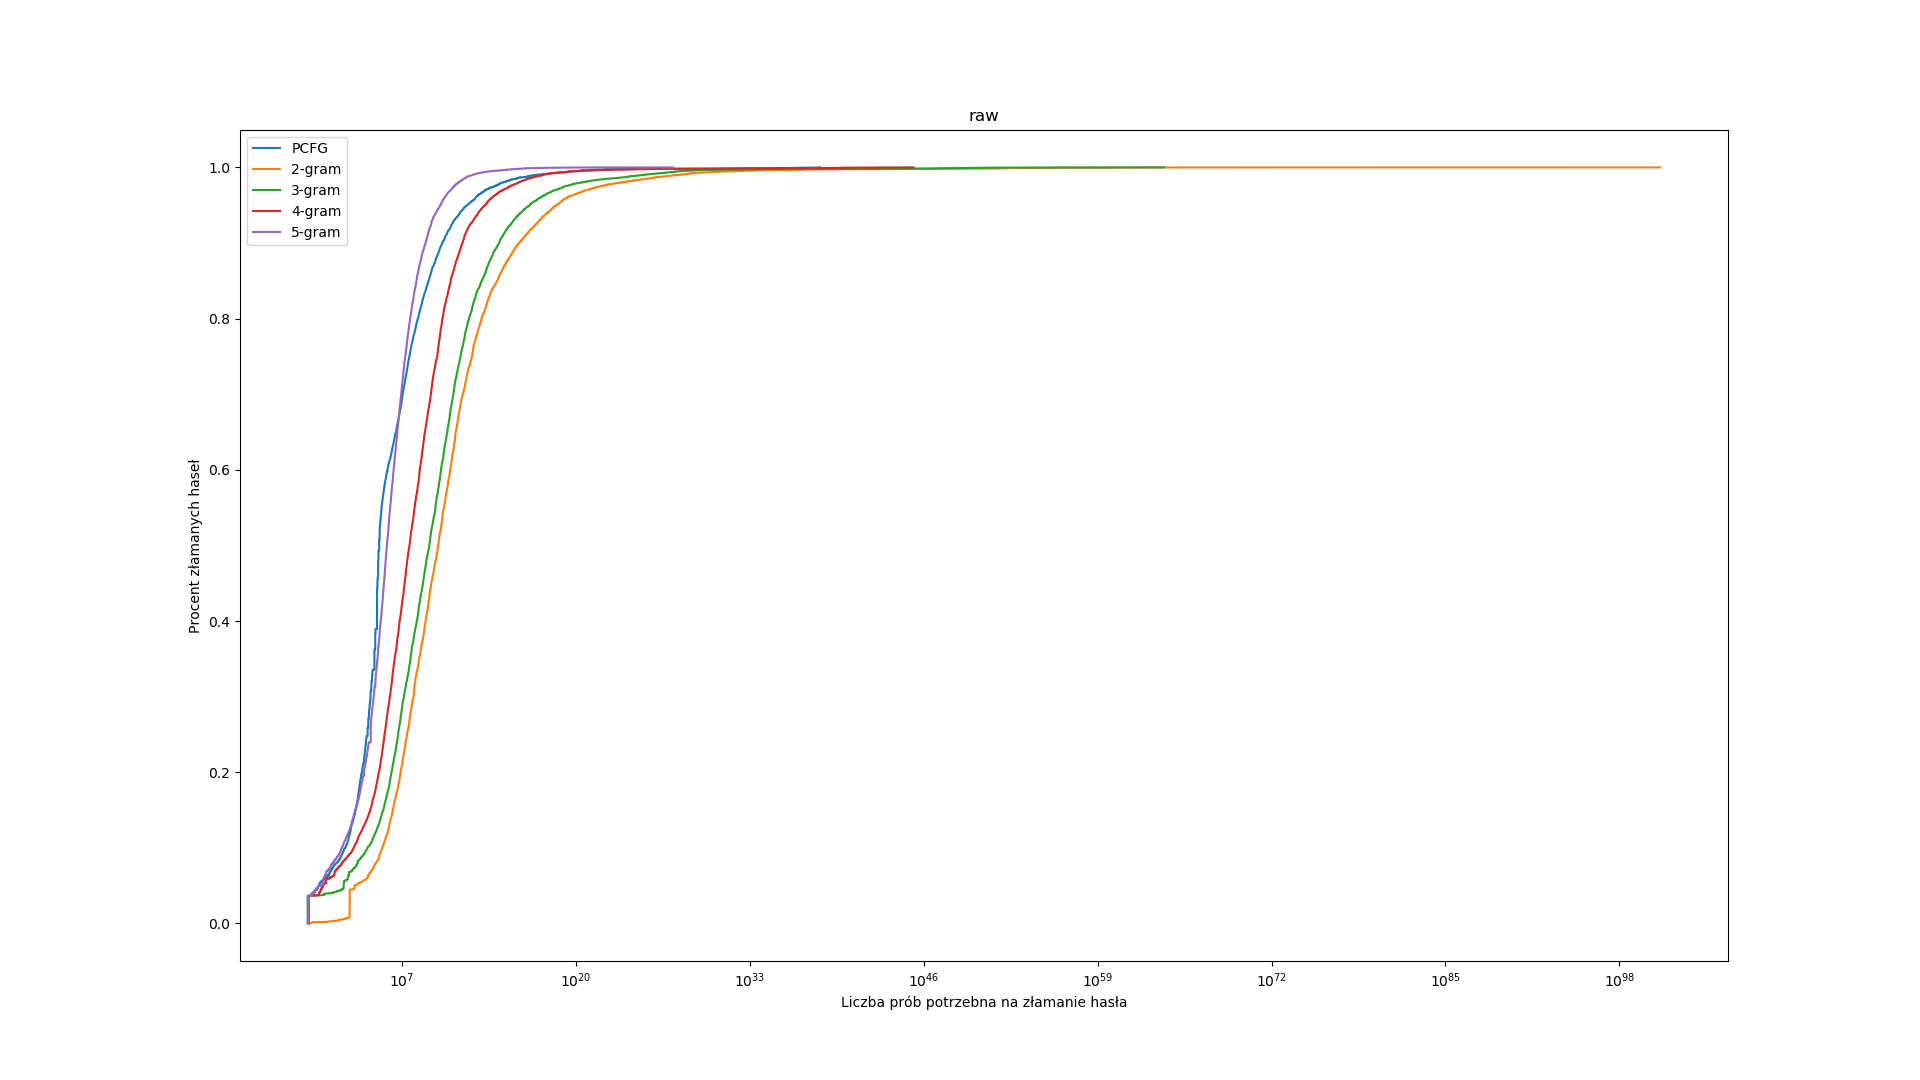
\includegraphics[width=15cm, keepaspectratio]{raw}
		\caption{Wpływ rodzaju algorytmu na liczbę prób potrzebnych do złamania haseł nienależących do żadnej polityki}
	\end{figure}

	\begin{figure}[H]
		\centering
		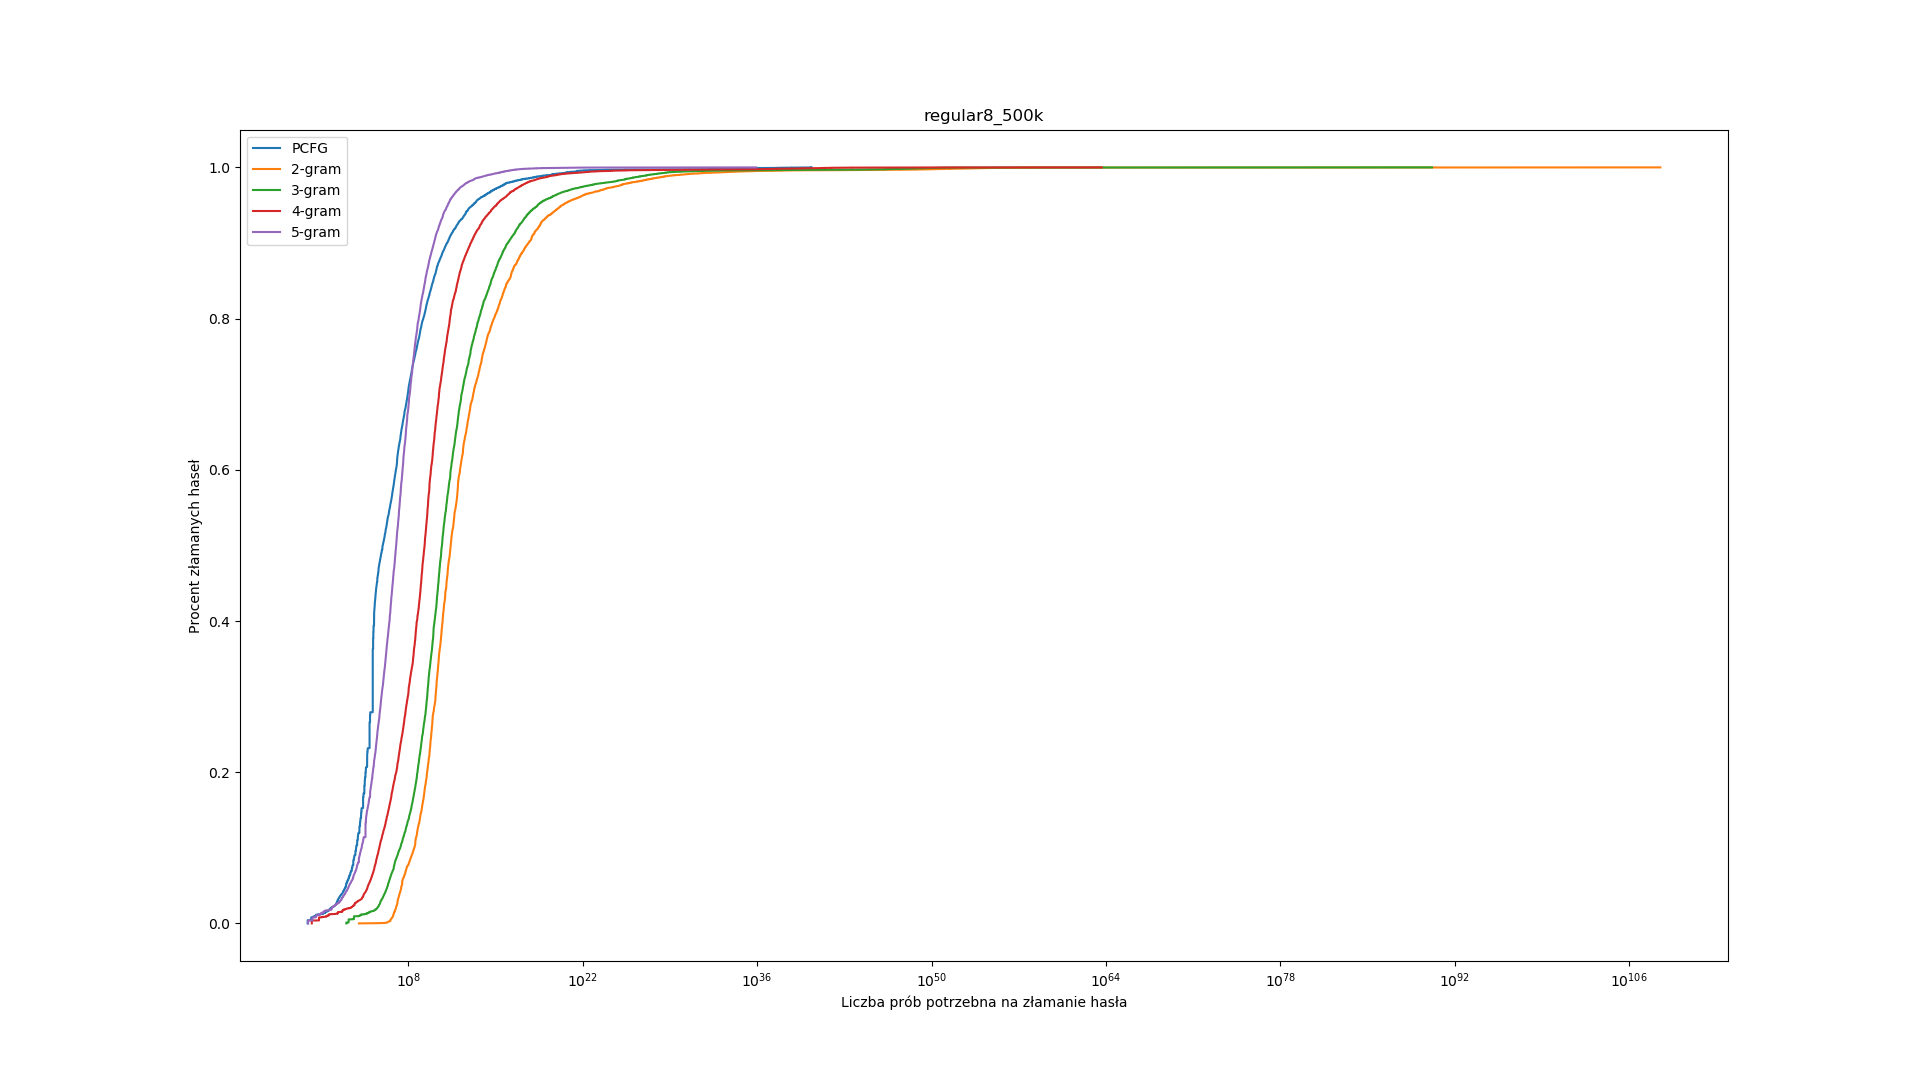
\includegraphics[width=15cm, keepaspectratio]{regular8_500k}
		\caption{Wpływ rodzaju algorytmu na liczbę prób potrzebnych do złamania haseł w polityce regular8 przy ciągu treningowym wielkośći 500 tysięcy haseł}
	\end{figure}

	\begin{figure}[H]
		\centering
		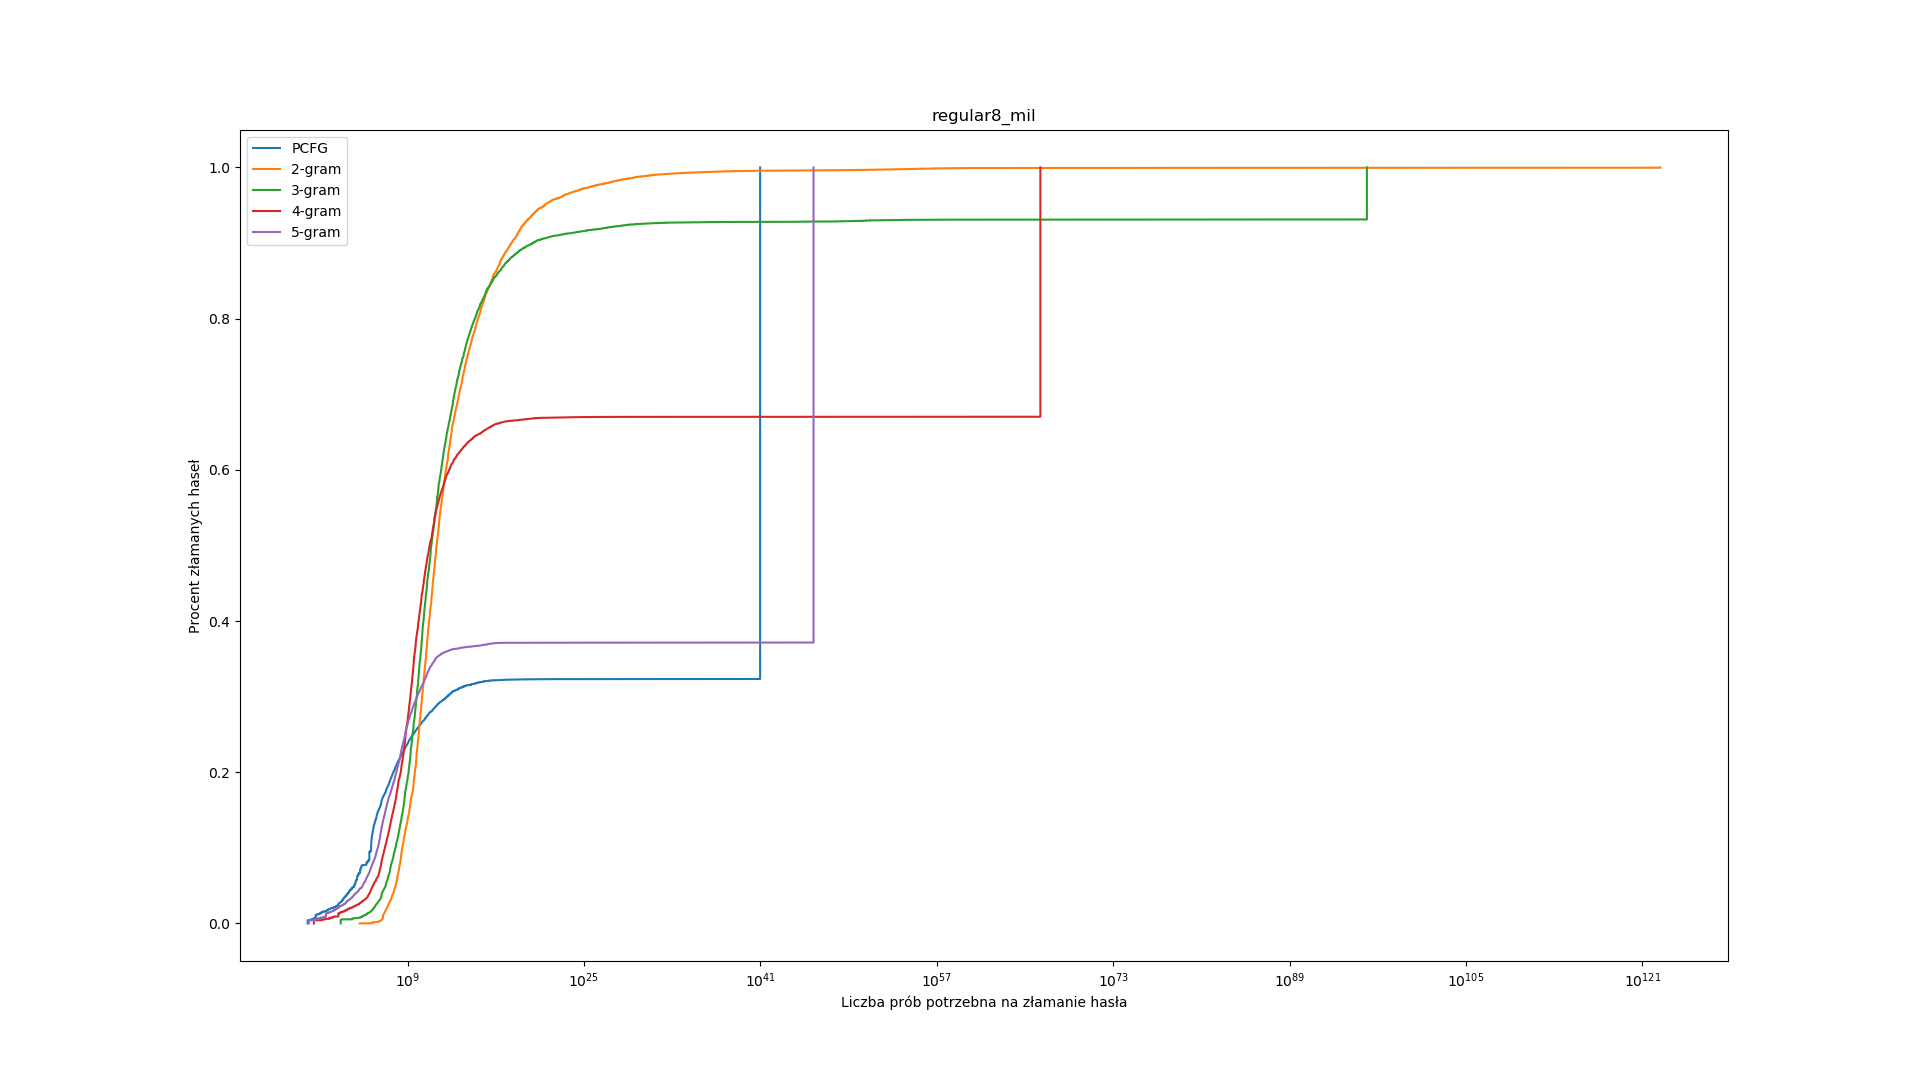
\includegraphics[width=15cm, keepaspectratio]{regular8_mil}
		\caption{Wpływ rodzaju algorytmu na liczbę prób potrzebnych do złamania haseł w polityce regular8 przy ciągu treningowym wielkośći miliona haseł}
	\end{figure}

	\begin{figure}[H]
		\centering
		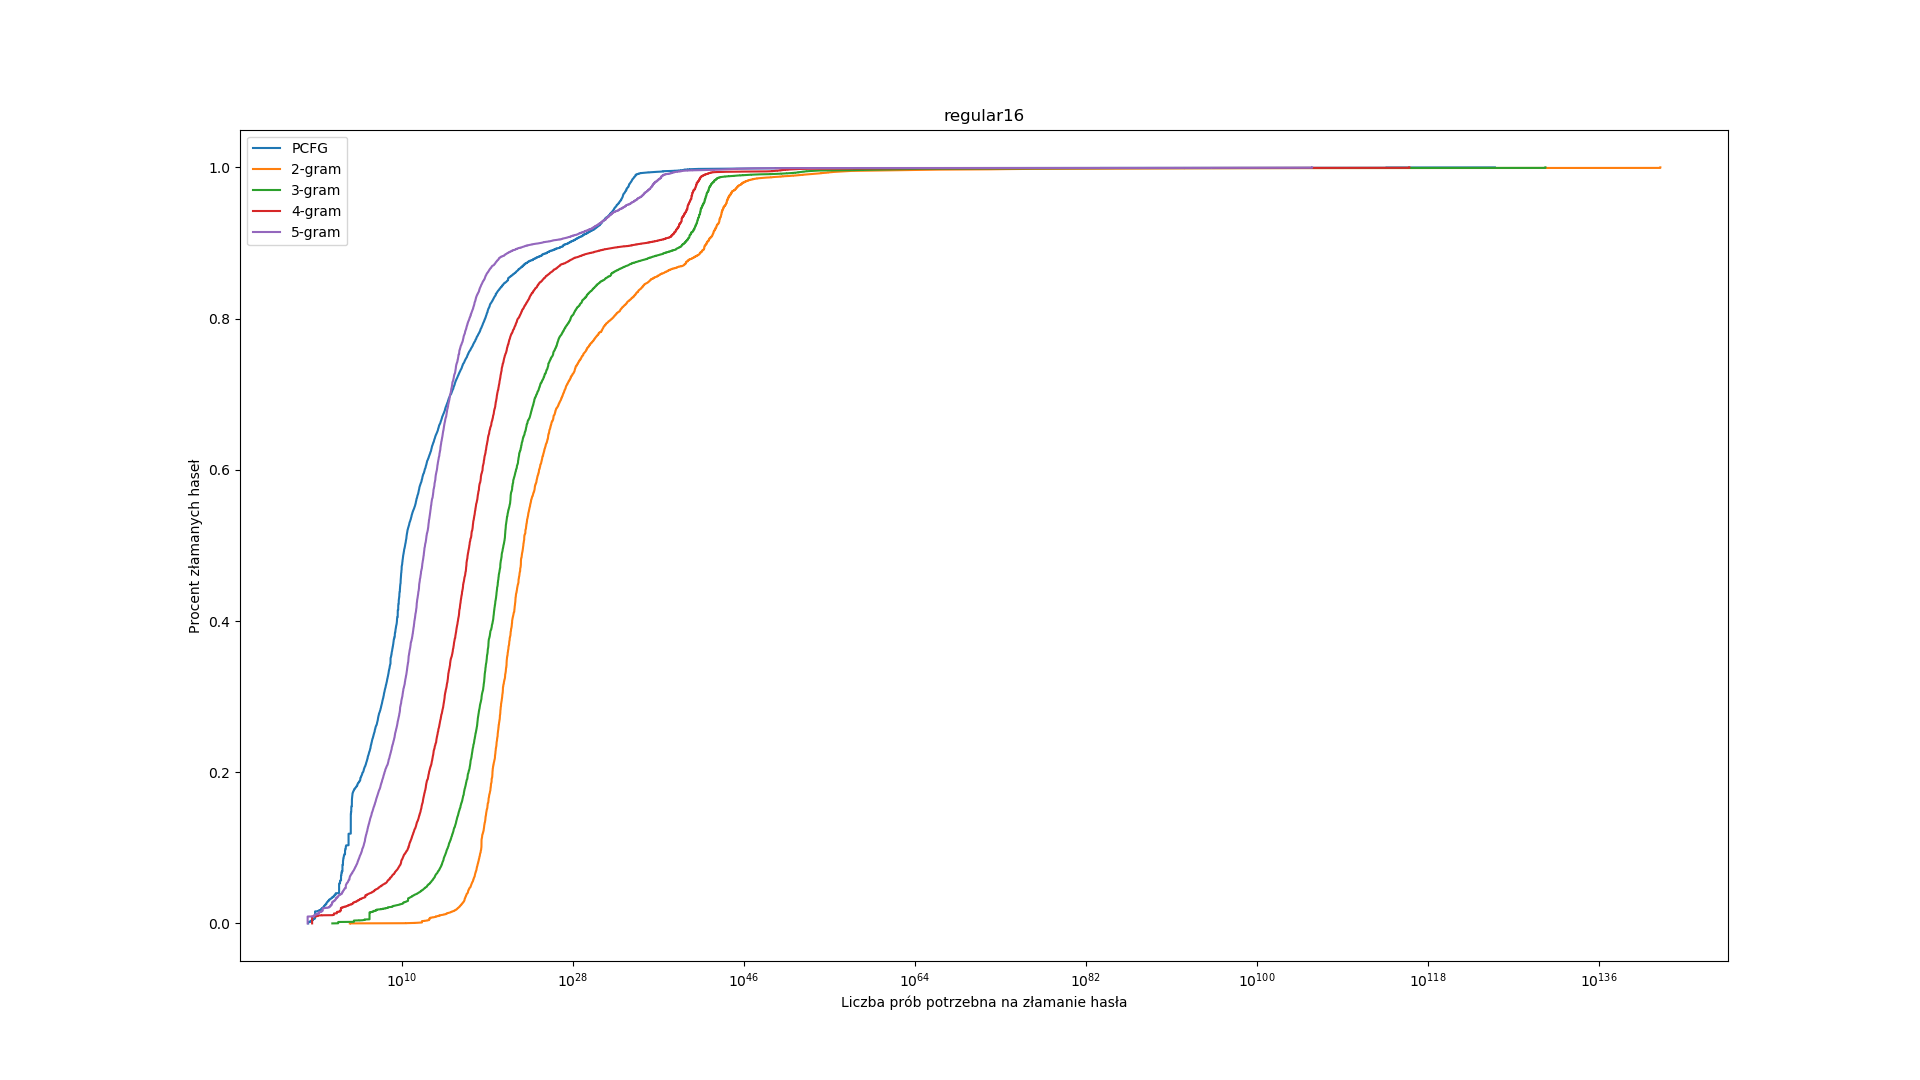
\includegraphics[width=15cm, keepaspectratio]{regular16}
		\caption{Wpływ rodzaju algorytmu na liczbę prób potrzebnych do złamania haseł w polityce regular16}
	\end{figure}

	\begin{figure}[H]
		\centering
		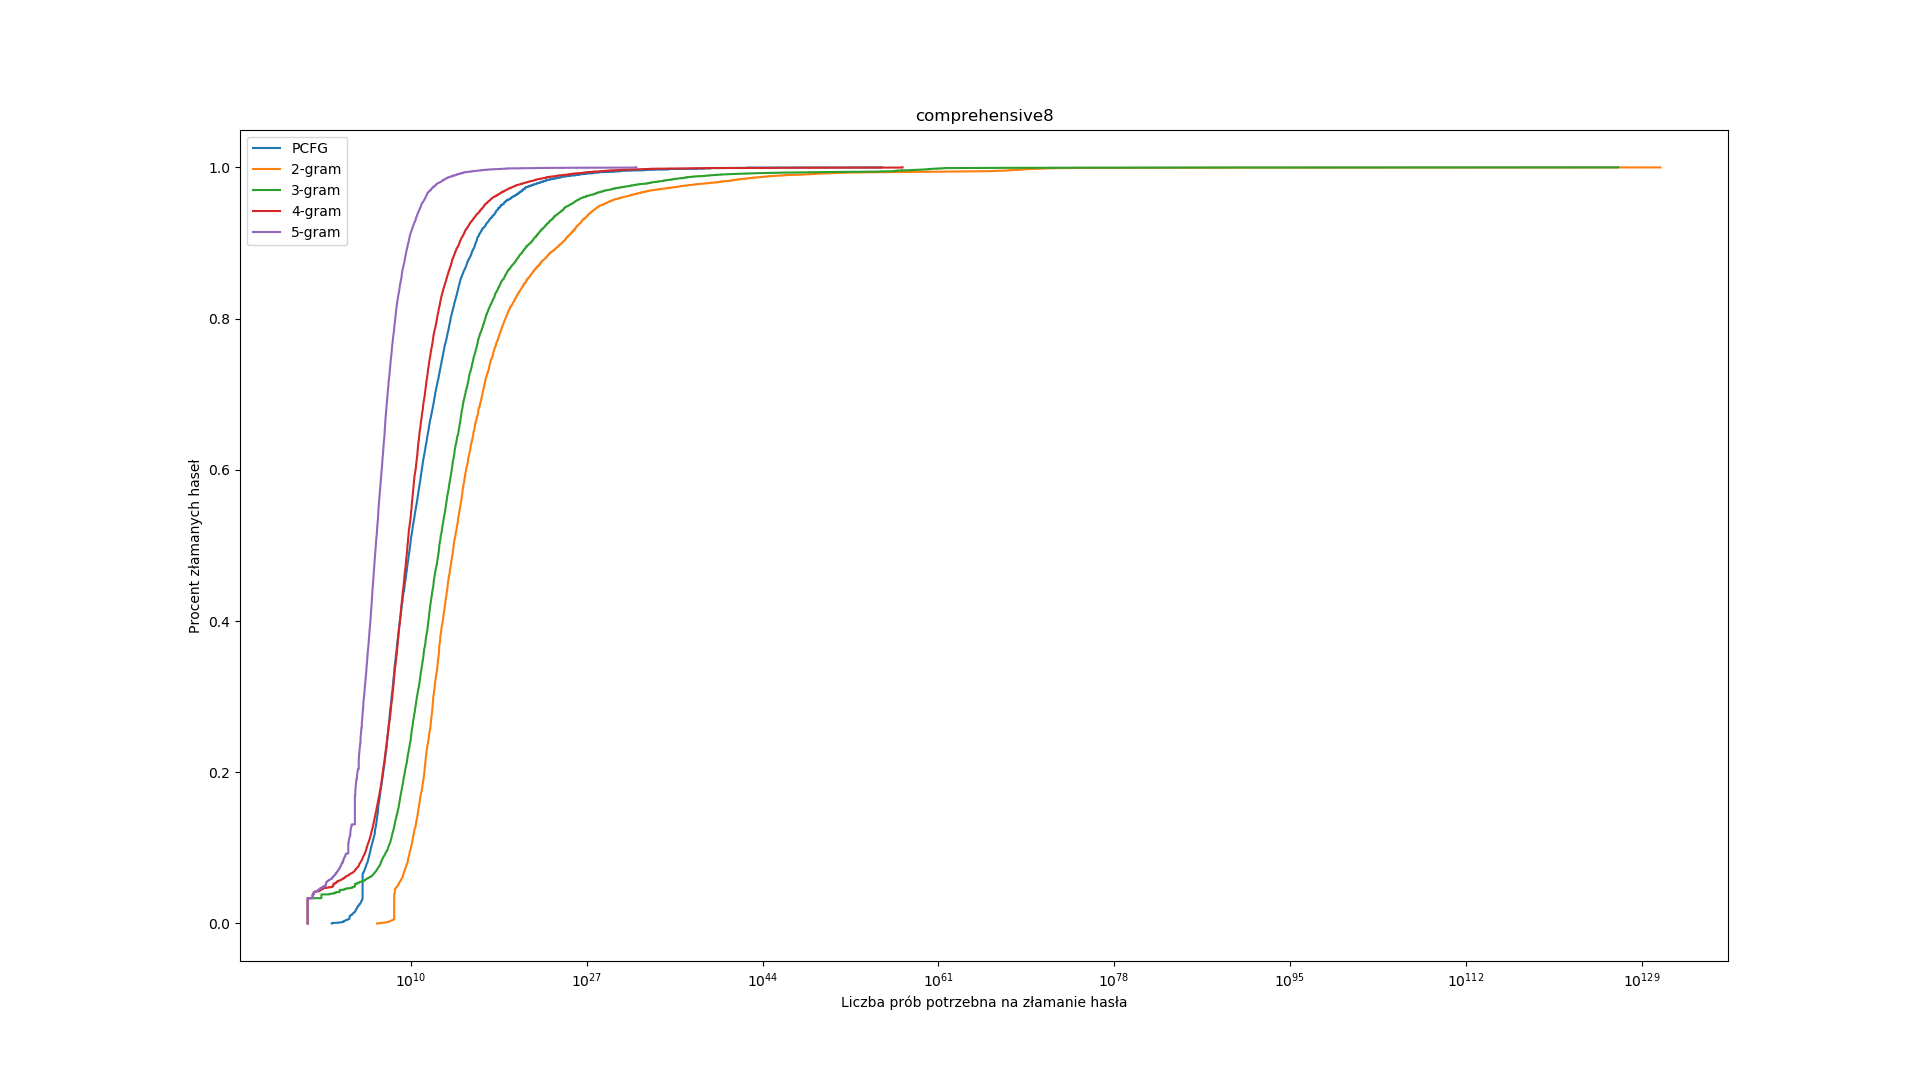
\includegraphics[width=15cm, keepaspectratio]{comprehensive8}
		\caption{Wpływ rodzaju algorytmu na liczbę prób potrzebnych do złamania haseł w polityce comprehensive8}
	\end{figure}

	\begin{figure}[H]
		\centering
		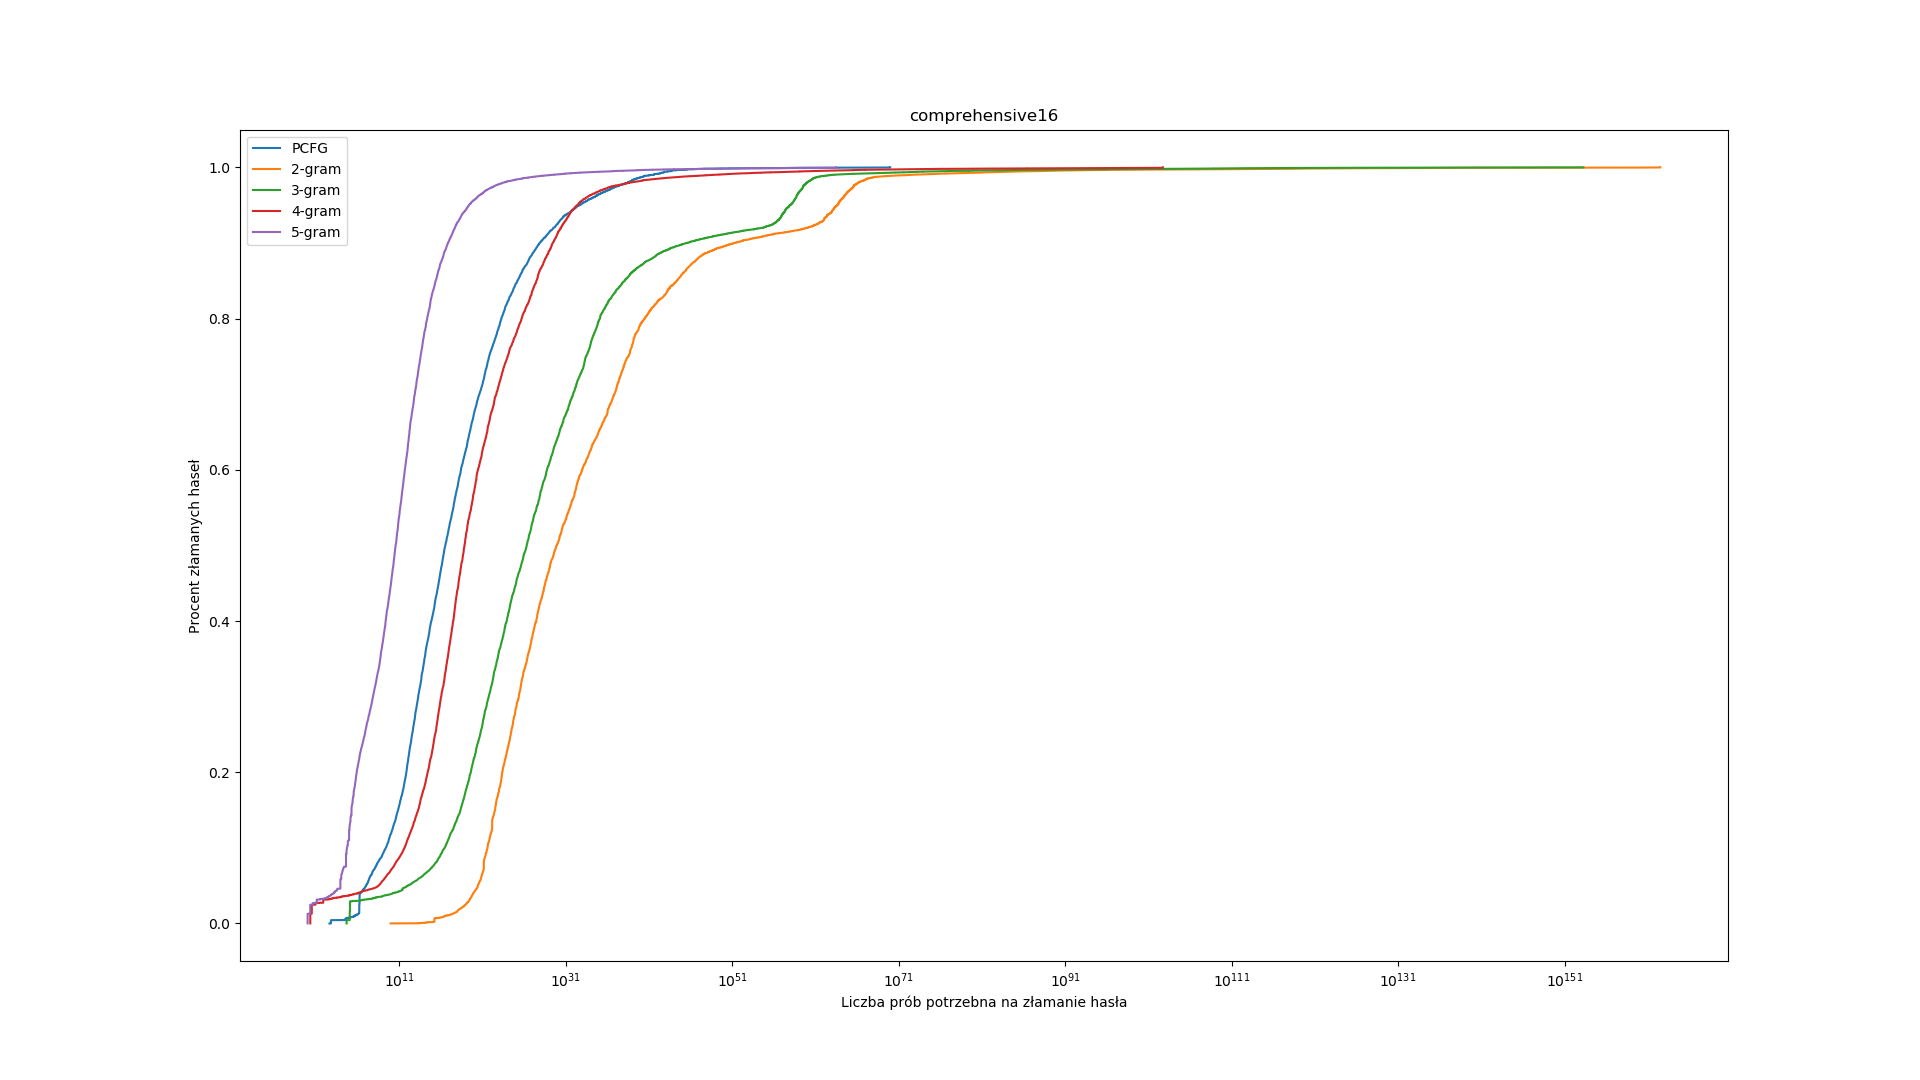
\includegraphics[width=15cm, keepaspectratio]{comprehensive16}
		\caption{Wpływ rodzaju algorytmu na liczbę prób potrzebnych do złamania haseł w polityce comprehensive16}
	\end{figure}

	\begin{figure}[H]
		\centering
		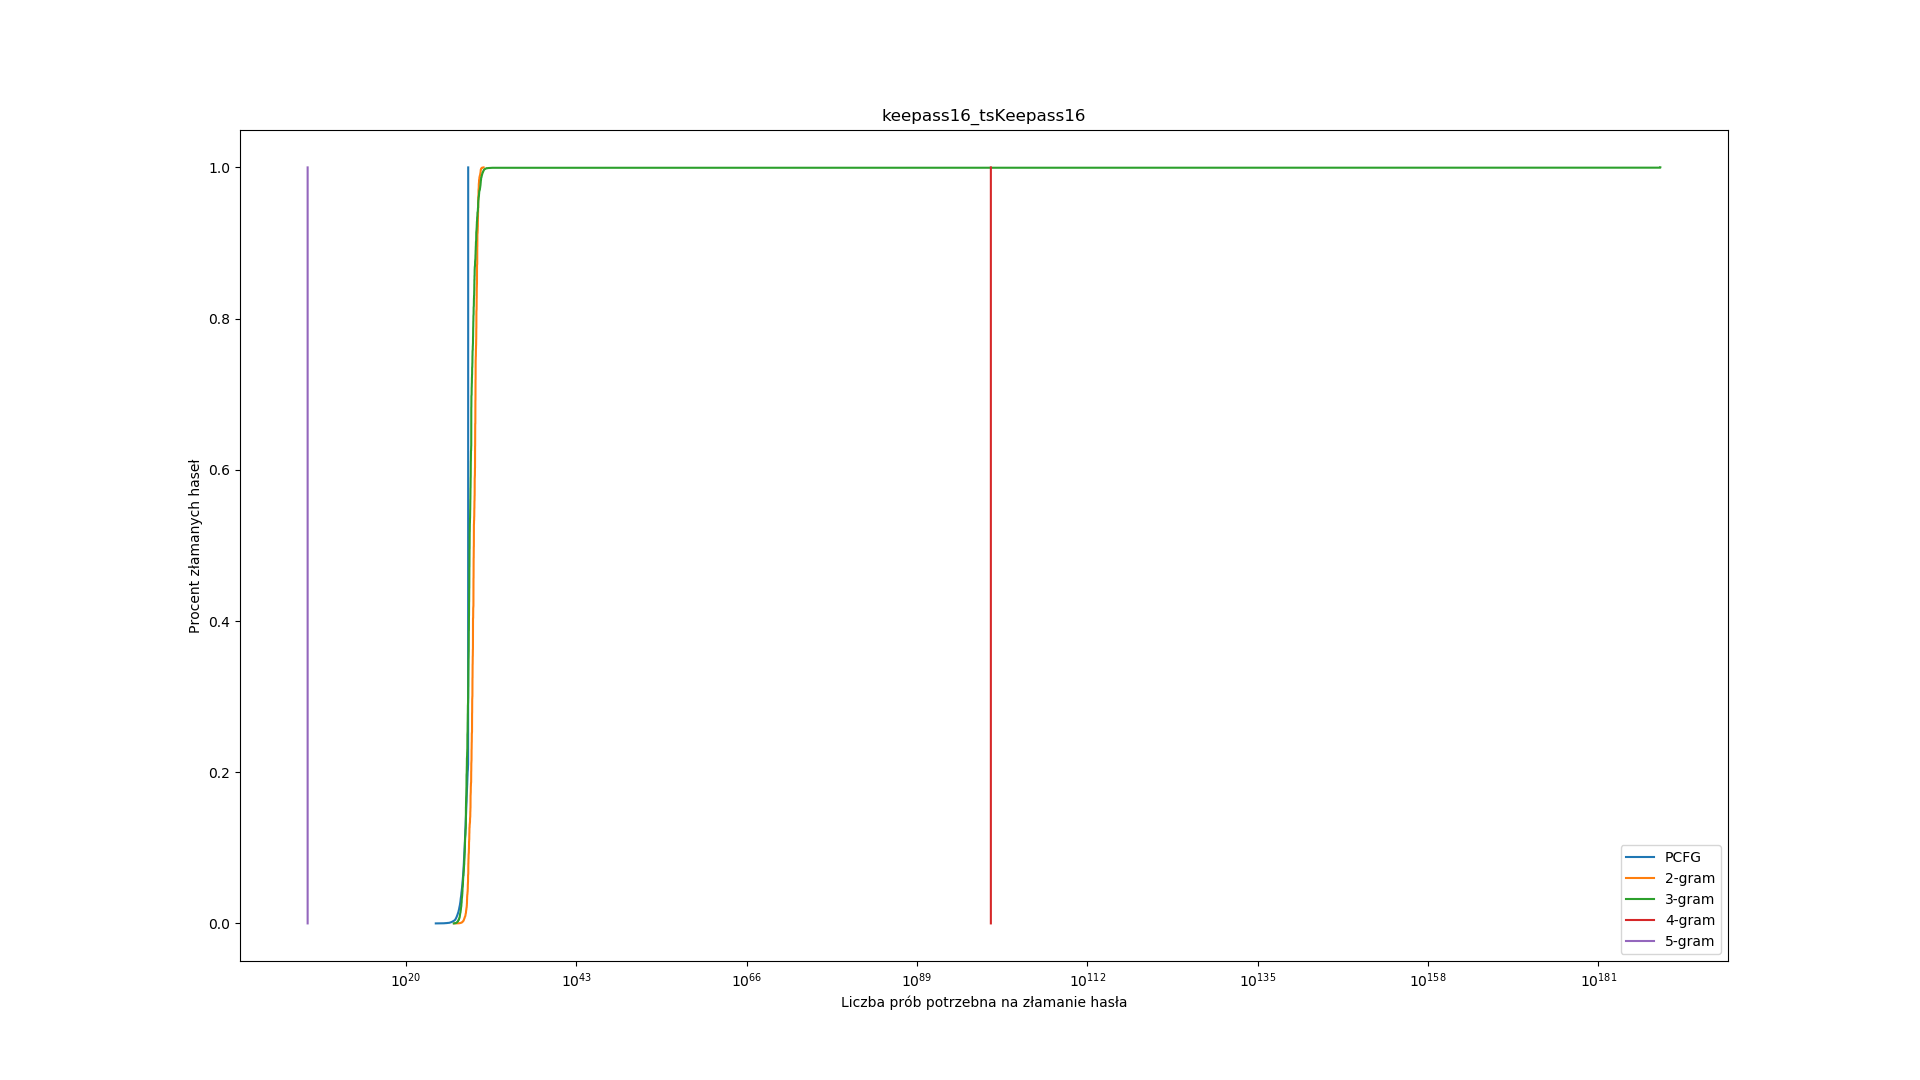
\includegraphics[width=15cm, keepaspectratio]{keepass16_tsKeepass16}
		\caption{Wpływ rodzaju algorytmu na liczbę prób potrzebnych do złamania haseł w polityce keepass16 przy ciągu treningowym złożonym z haseł w polityce keepass16}
	\end{figure}

	\begin{figure}[H]
		\centering
		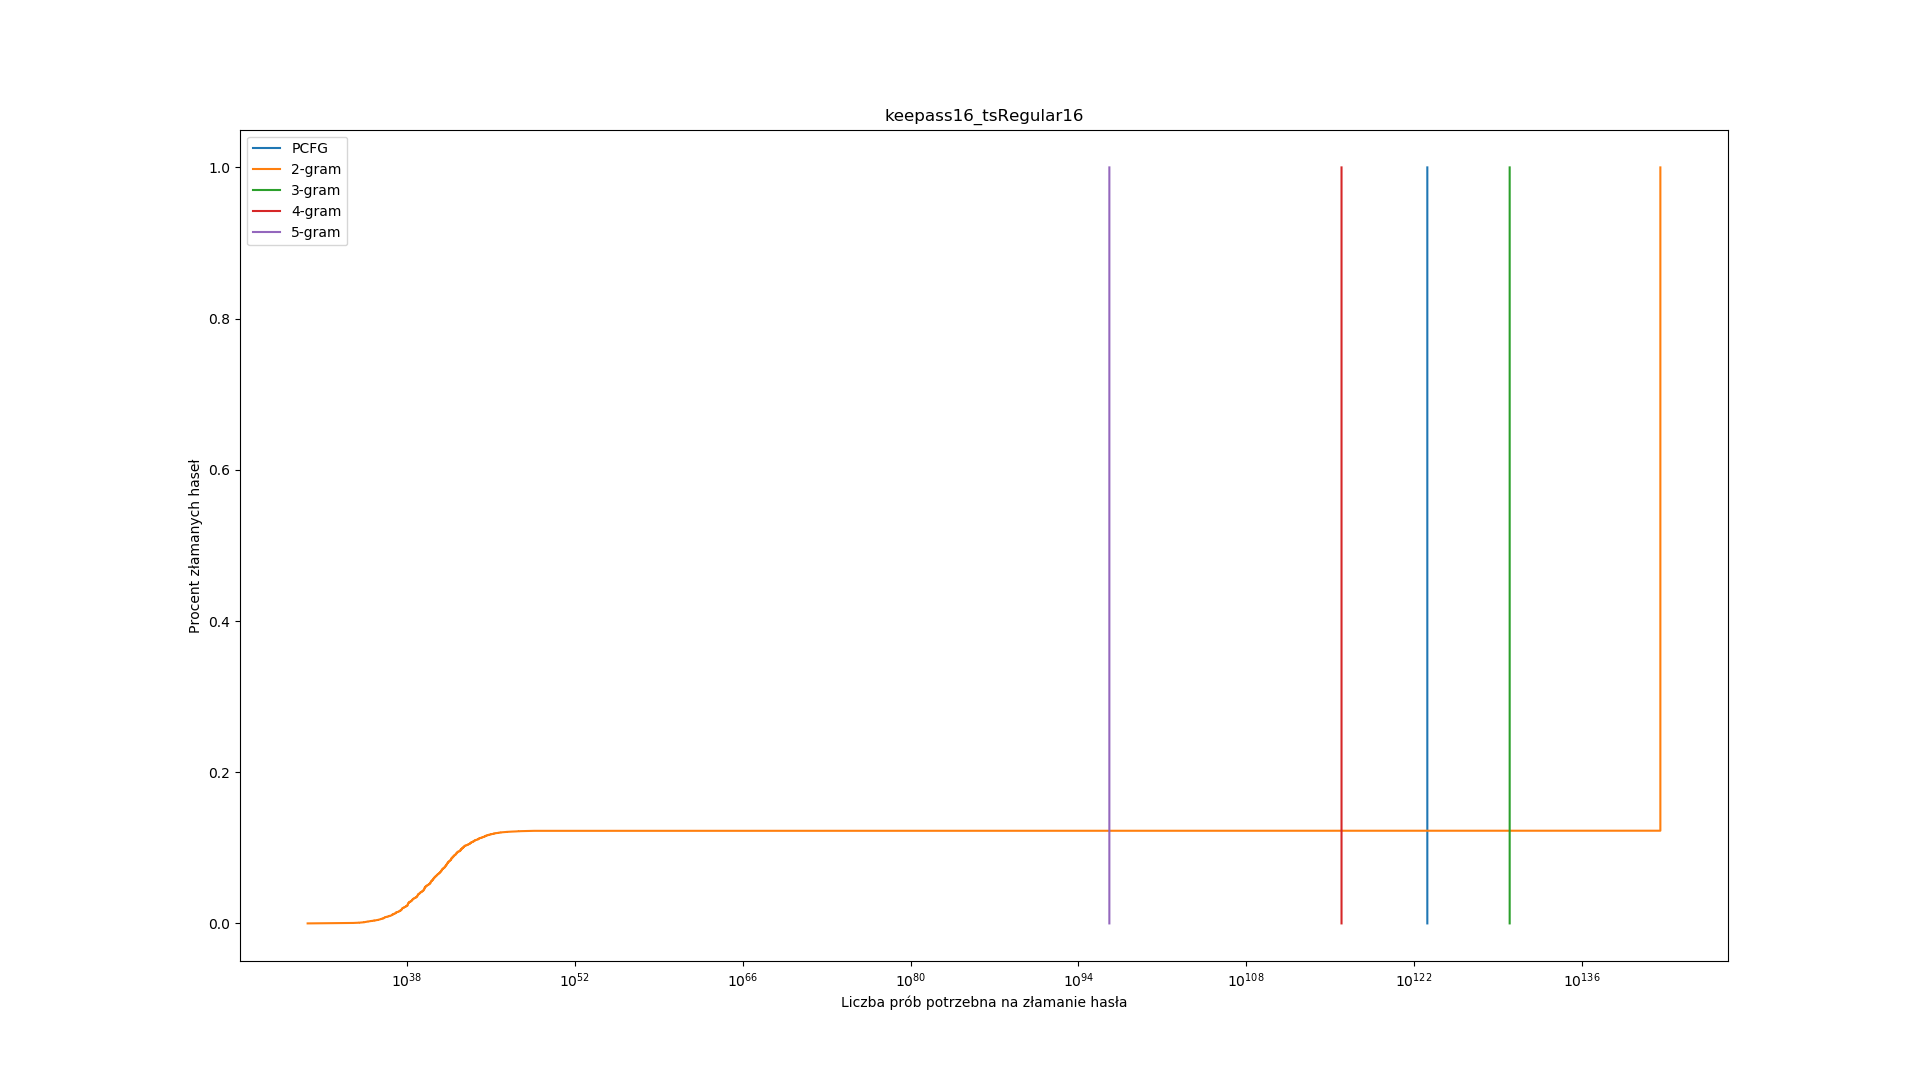
\includegraphics[width=15cm, keepaspectratio]{keepass16_tsRegular16}
		\caption{Wpływ rodzaju algorytmu na liczbę prób potrzebnych do złamania haseł w polityce keepass16 przy ciągu treningowym złożonym z haseł w polityce regular16}
	\end{figure}


	Rysunki 1 - 8 przedstawiają ile faktycznych prób musi wykonać każdy z algorytmów, aby odgadnąć procentową część wszystkich haseł z ciągu walidacyjnego.

	\subsection{Porównanie wpływu rodzaju algorytmu na skuteczność łamania haseł w każdej z polityk}
	\begin{figure}[H]
		\centering
		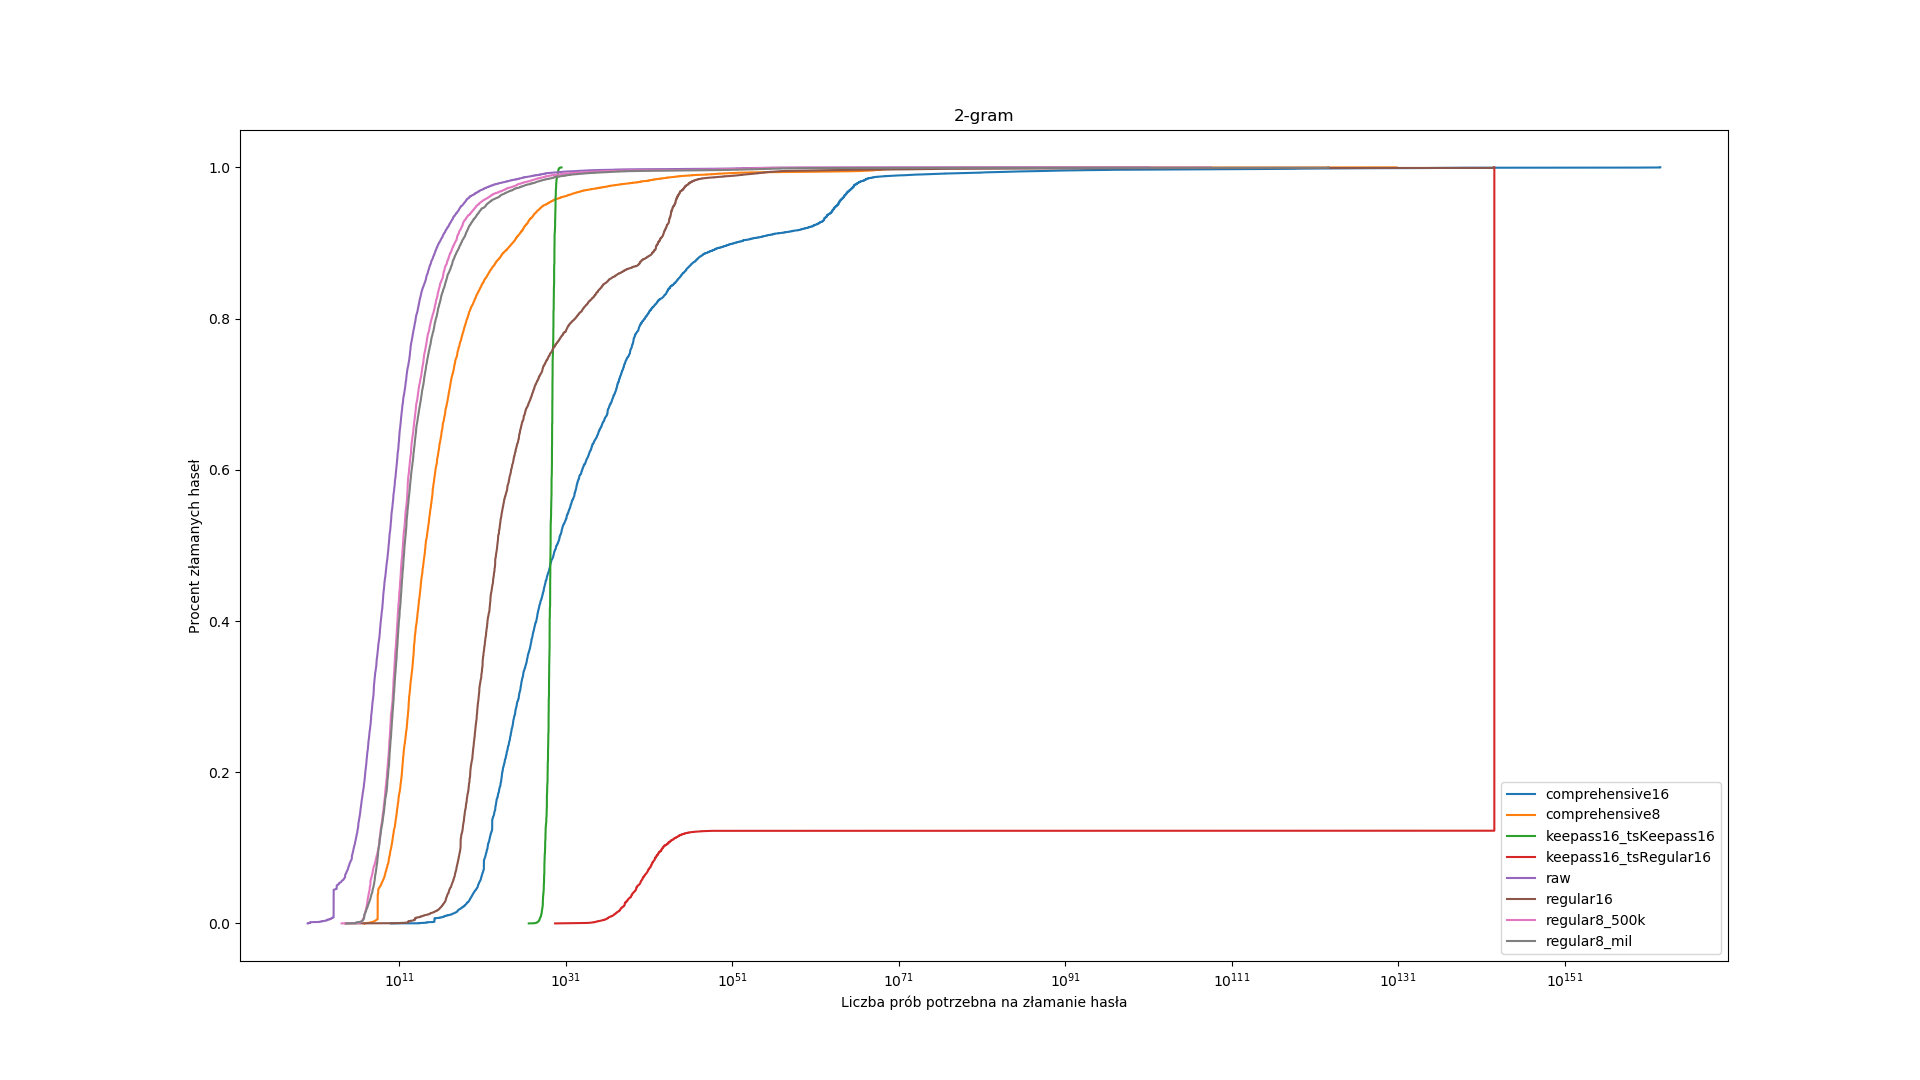
\includegraphics[width=15cm, keepaspectratio]{2-gram}
		\caption{Skuteczność łamania haseł dla każdej polityki w algorytmie bazującym na 2-gramach (standardowy BFM)}
	\end{figure}

	\begin{figure}[H]
		\centering
		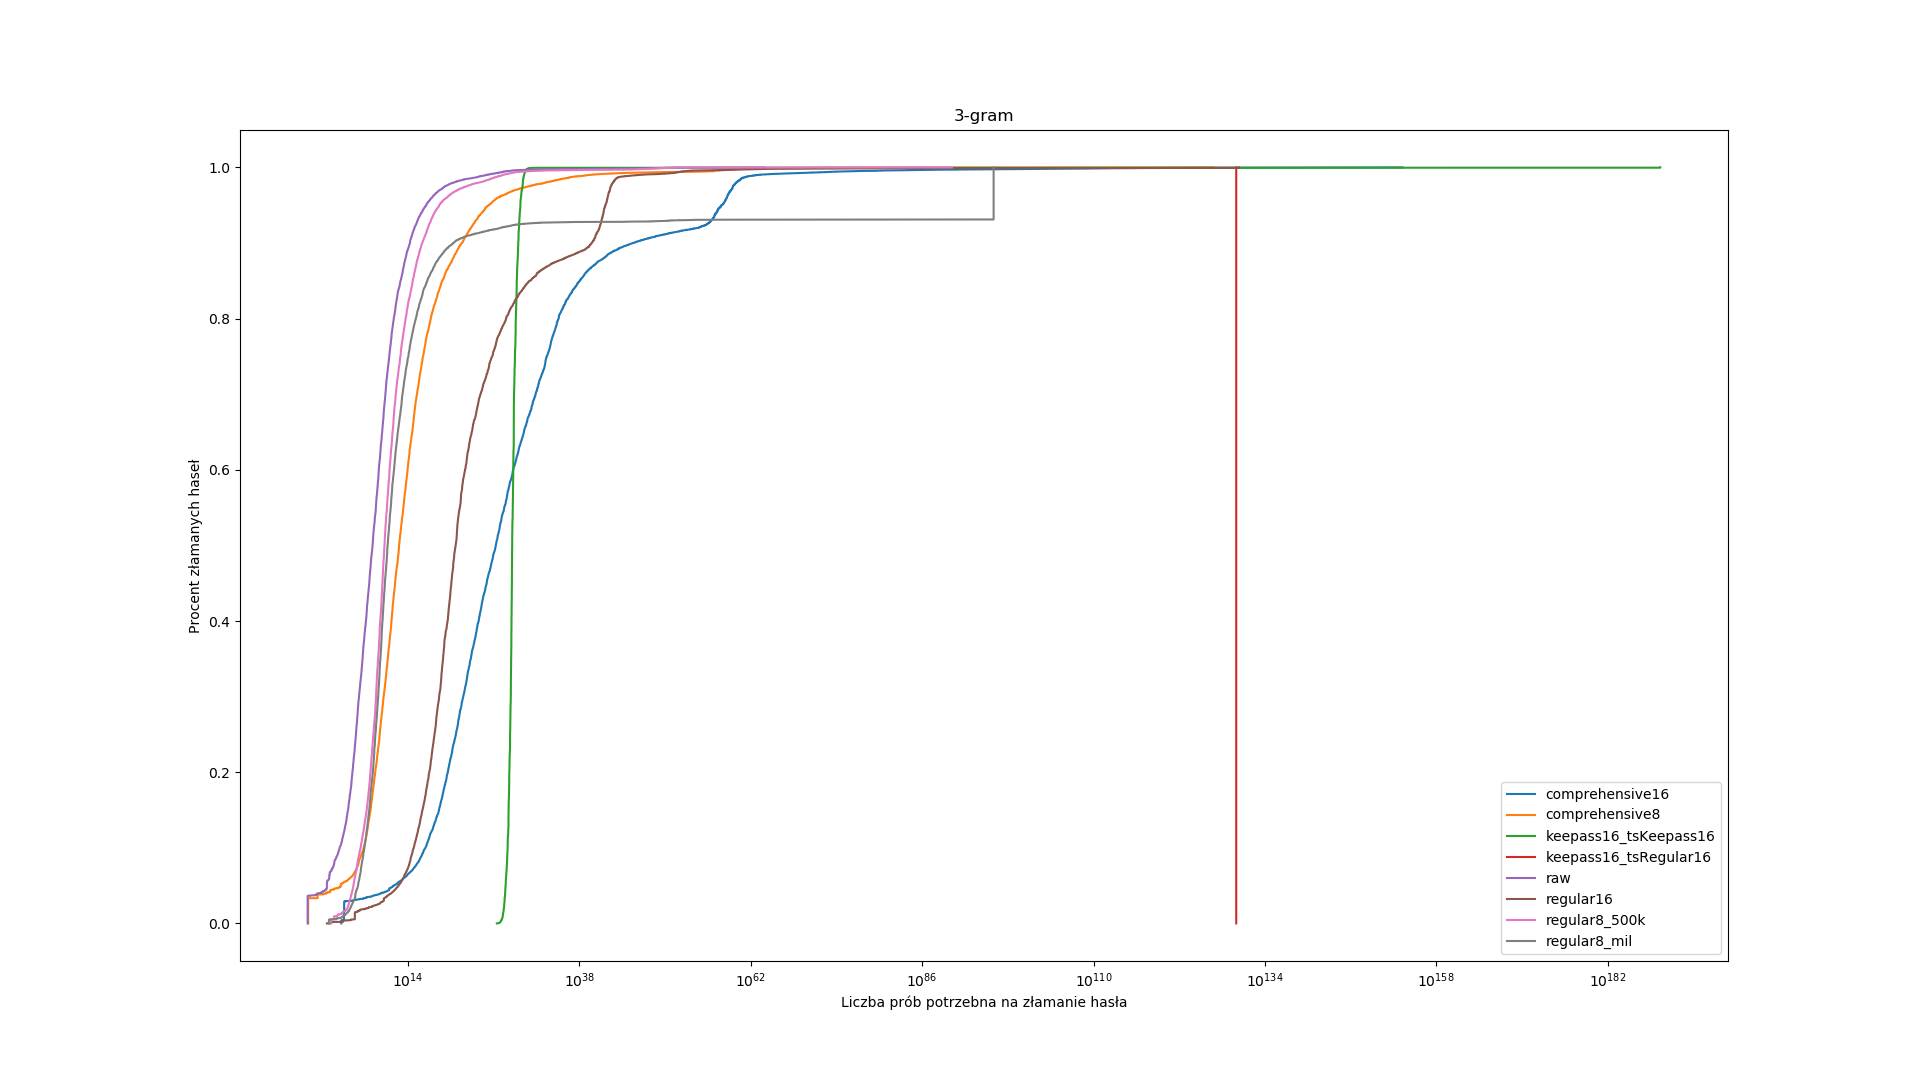
\includegraphics[width=15cm, keepaspectratio]{3-gram}
		\caption{Skuteczność łamania haseł dla każdej polityki w algorytmie bazującym na 3-gramach}
	\end{figure}

	\begin{figure}[H]
		\centering
		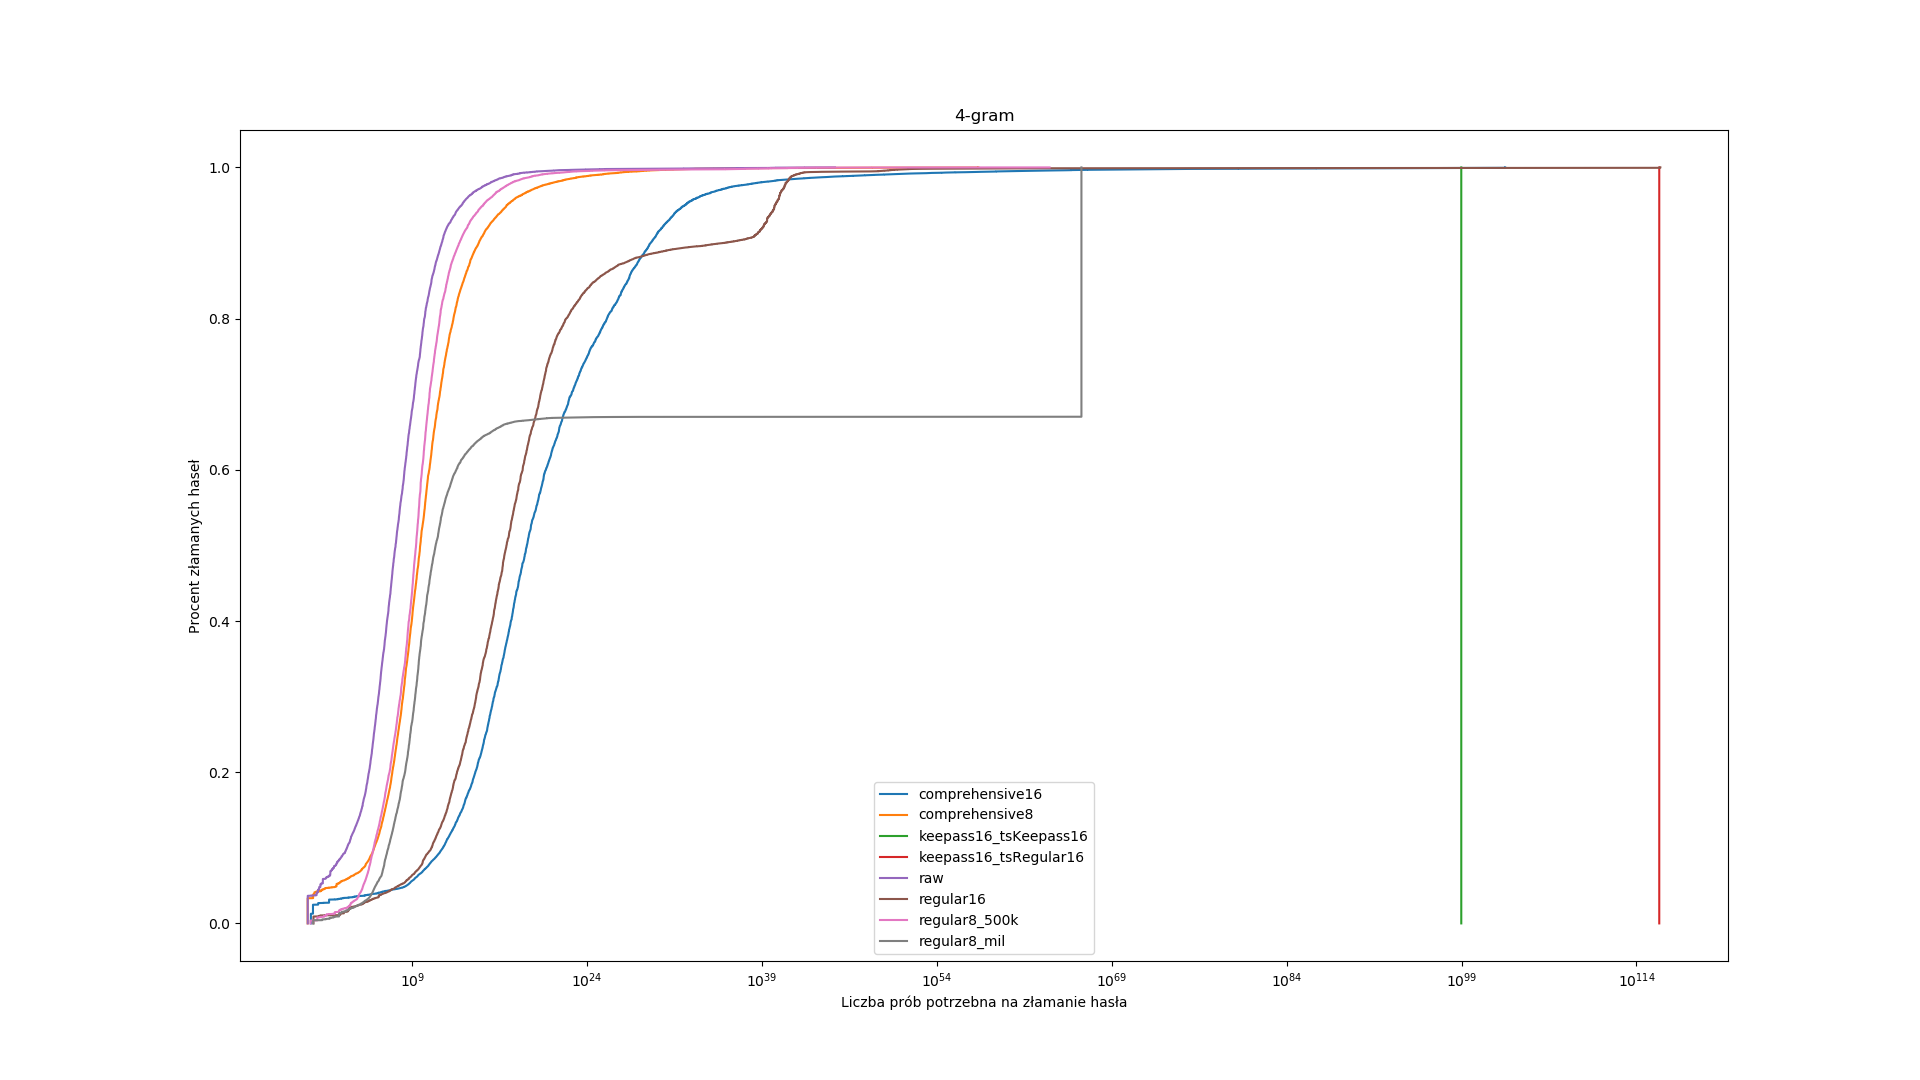
\includegraphics[width=15cm, keepaspectratio]{4-gram}
		\caption{Skuteczność łamania haseł dla każdej polityki w algorytmie bazującym na 4-gramach}
	\end{figure}

	\begin{figure}[H]
		\centering
		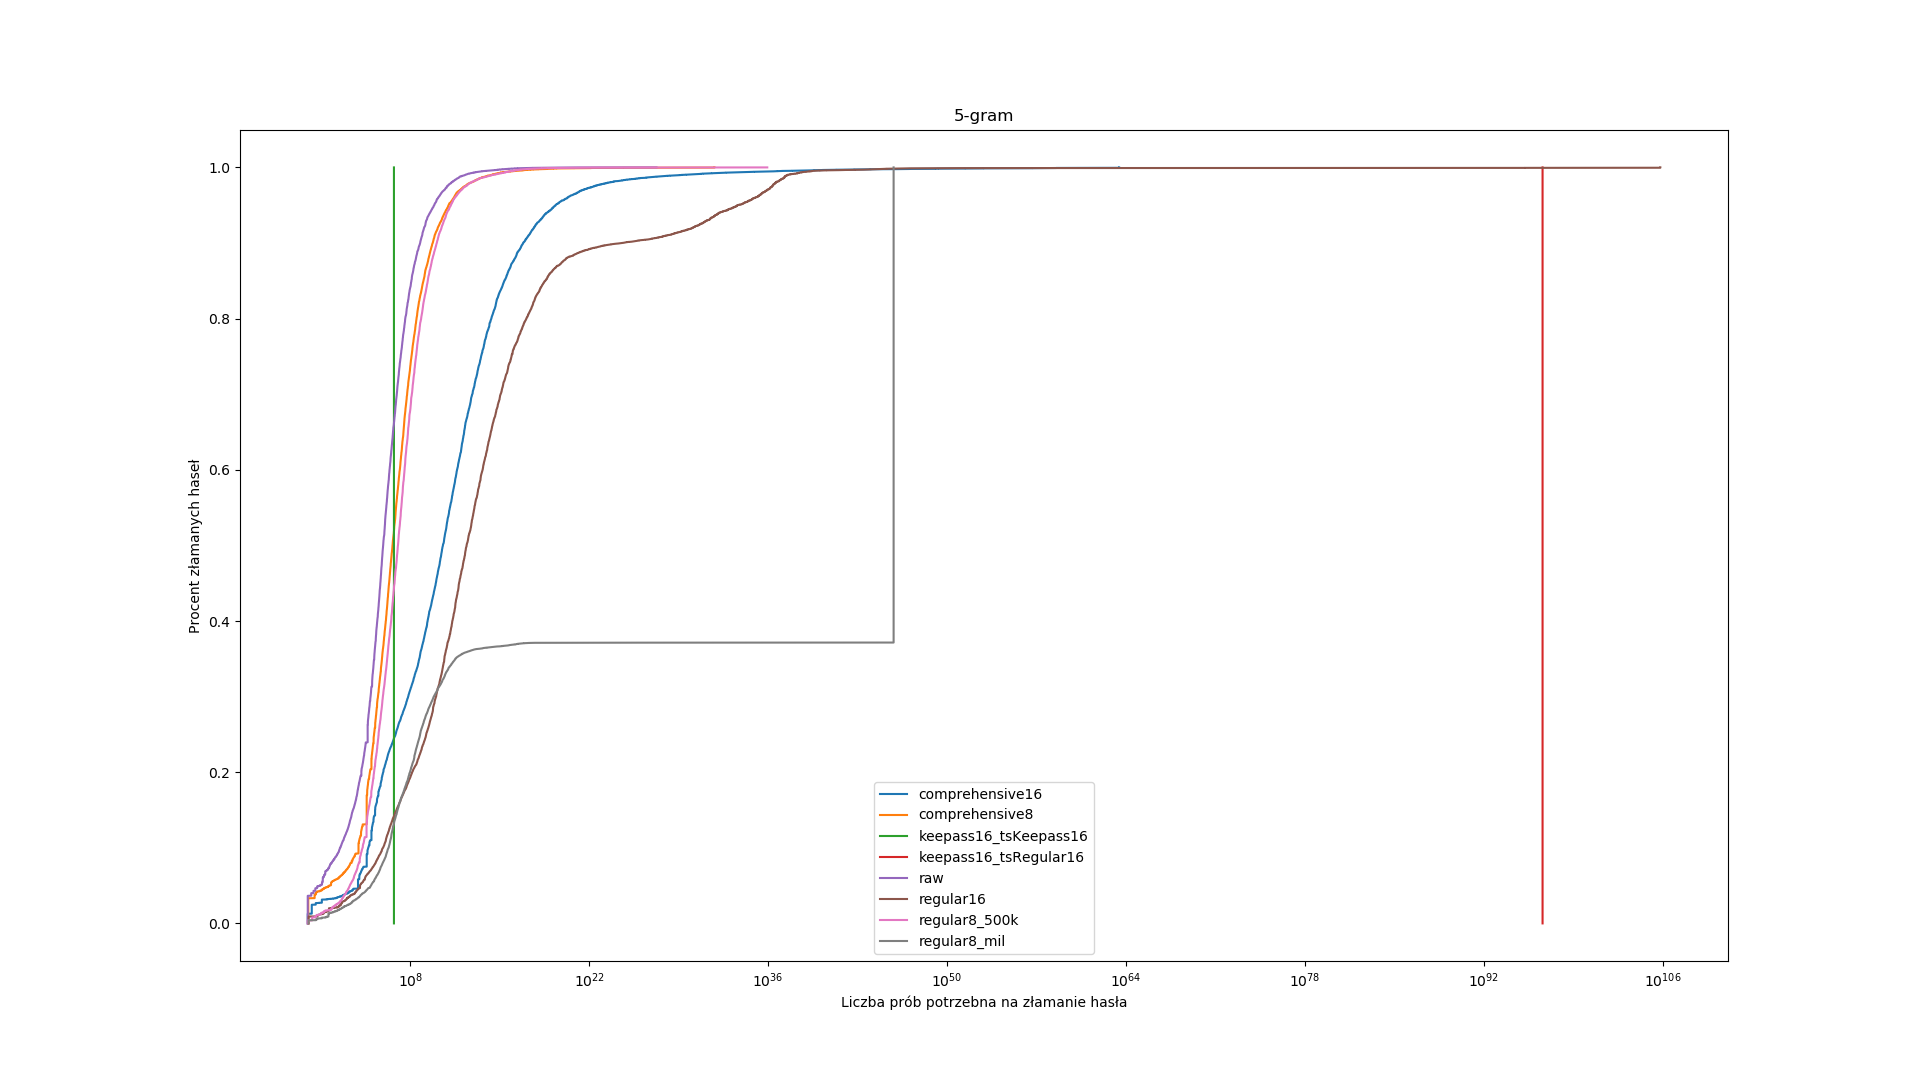
\includegraphics[width=15cm, keepaspectratio]{5-gram}
		\caption{Skuteczność łamania haseł dla każdej polityki w algorytmie bazującym na 5-gramach}
	\end{figure}

	\begin{figure}[H]
		\centering
		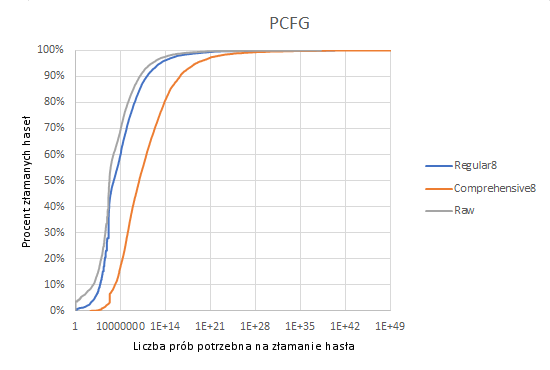
\includegraphics[width=15cm, keepaspectratio]{PCFG}
		\caption{Skuteczność łamania haseł dla każdej polityki w algorytmie PCFG (algorytmie Weira)}
	\end{figure}

	Rysunki 9-13 przedstawiają liczbę prób potrzebną do złamania procentowej części wszystkich haseł z ciągu walidacyjnego.

	\subsection{Porównanie poszczególnych polityk}
	\begin{figure}[H]
		\centering
		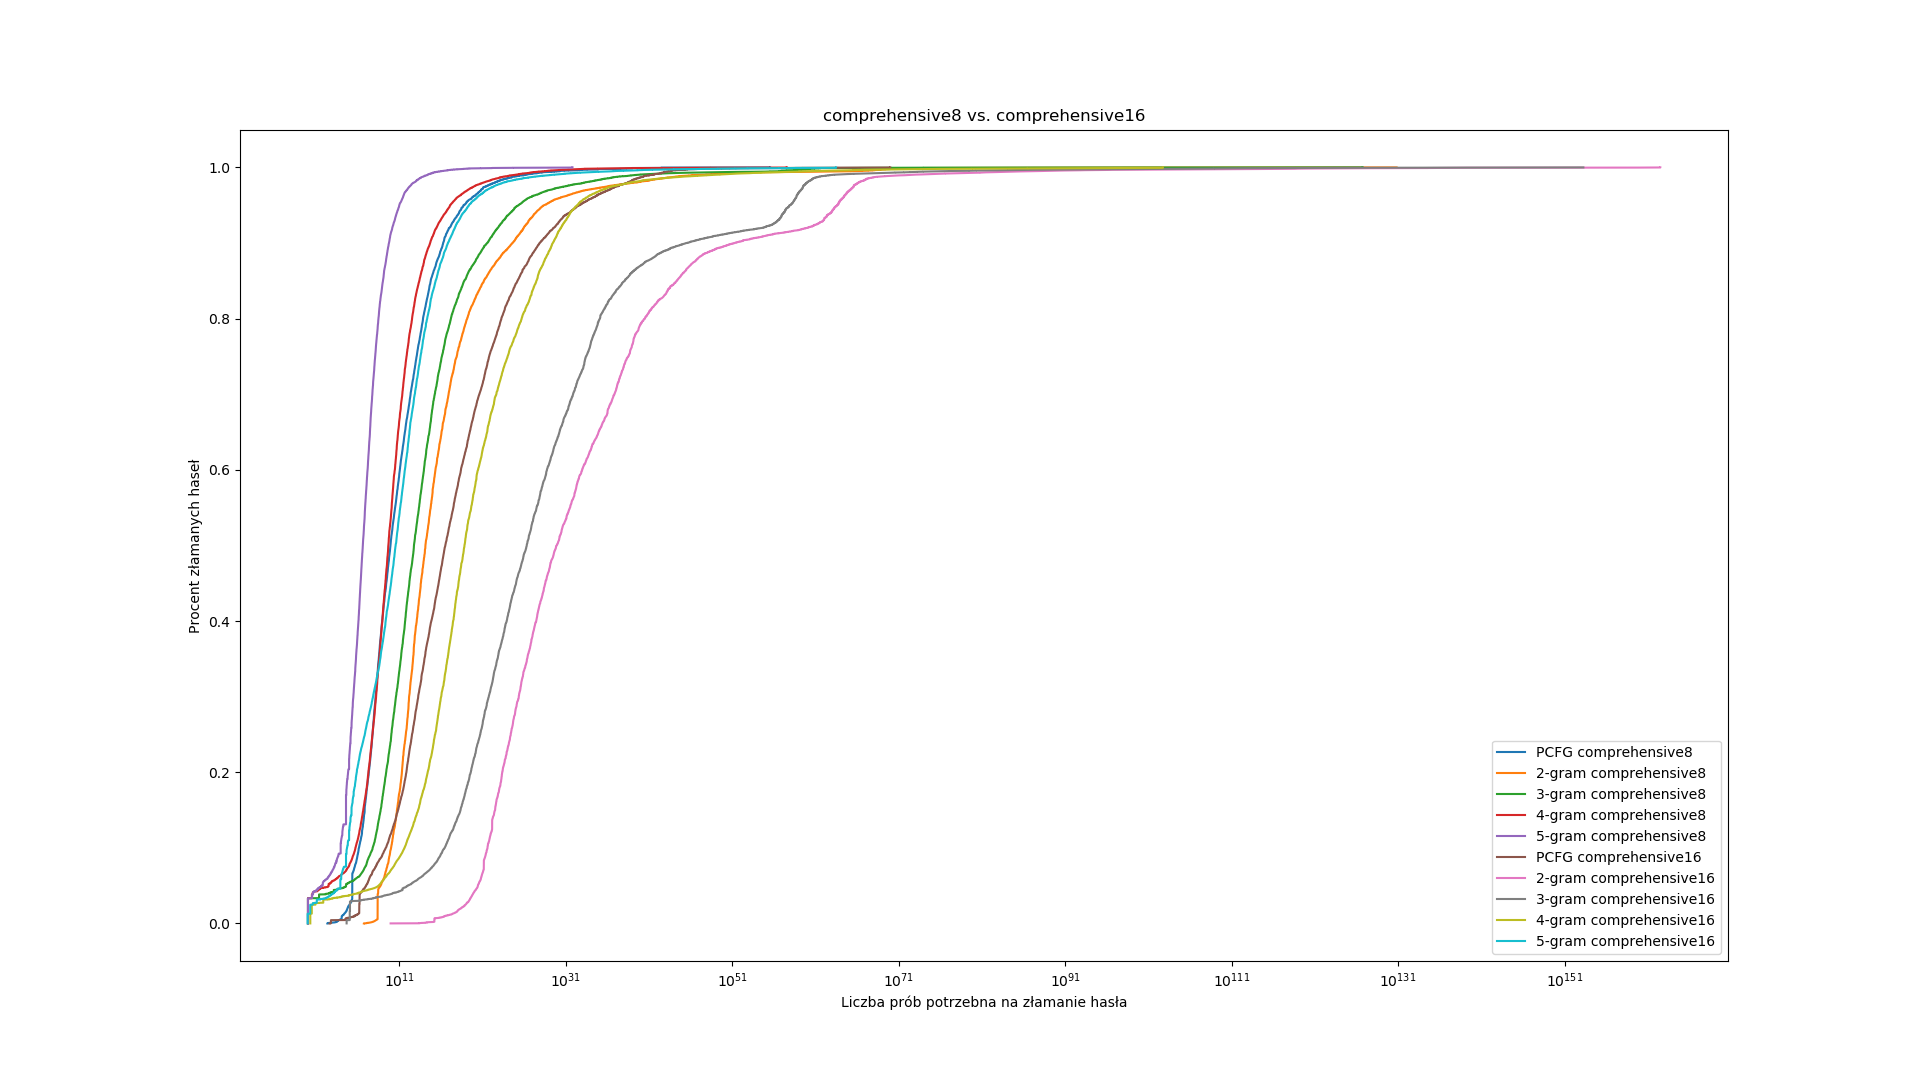
\includegraphics[width=15cm, keepaspectratio]{comprehensive8_comprehensive16}
		\caption{Porównanie polityki comprehensive8 i comprehensive16}
	\end{figure}

	\begin{figure}[H]
		\centering
		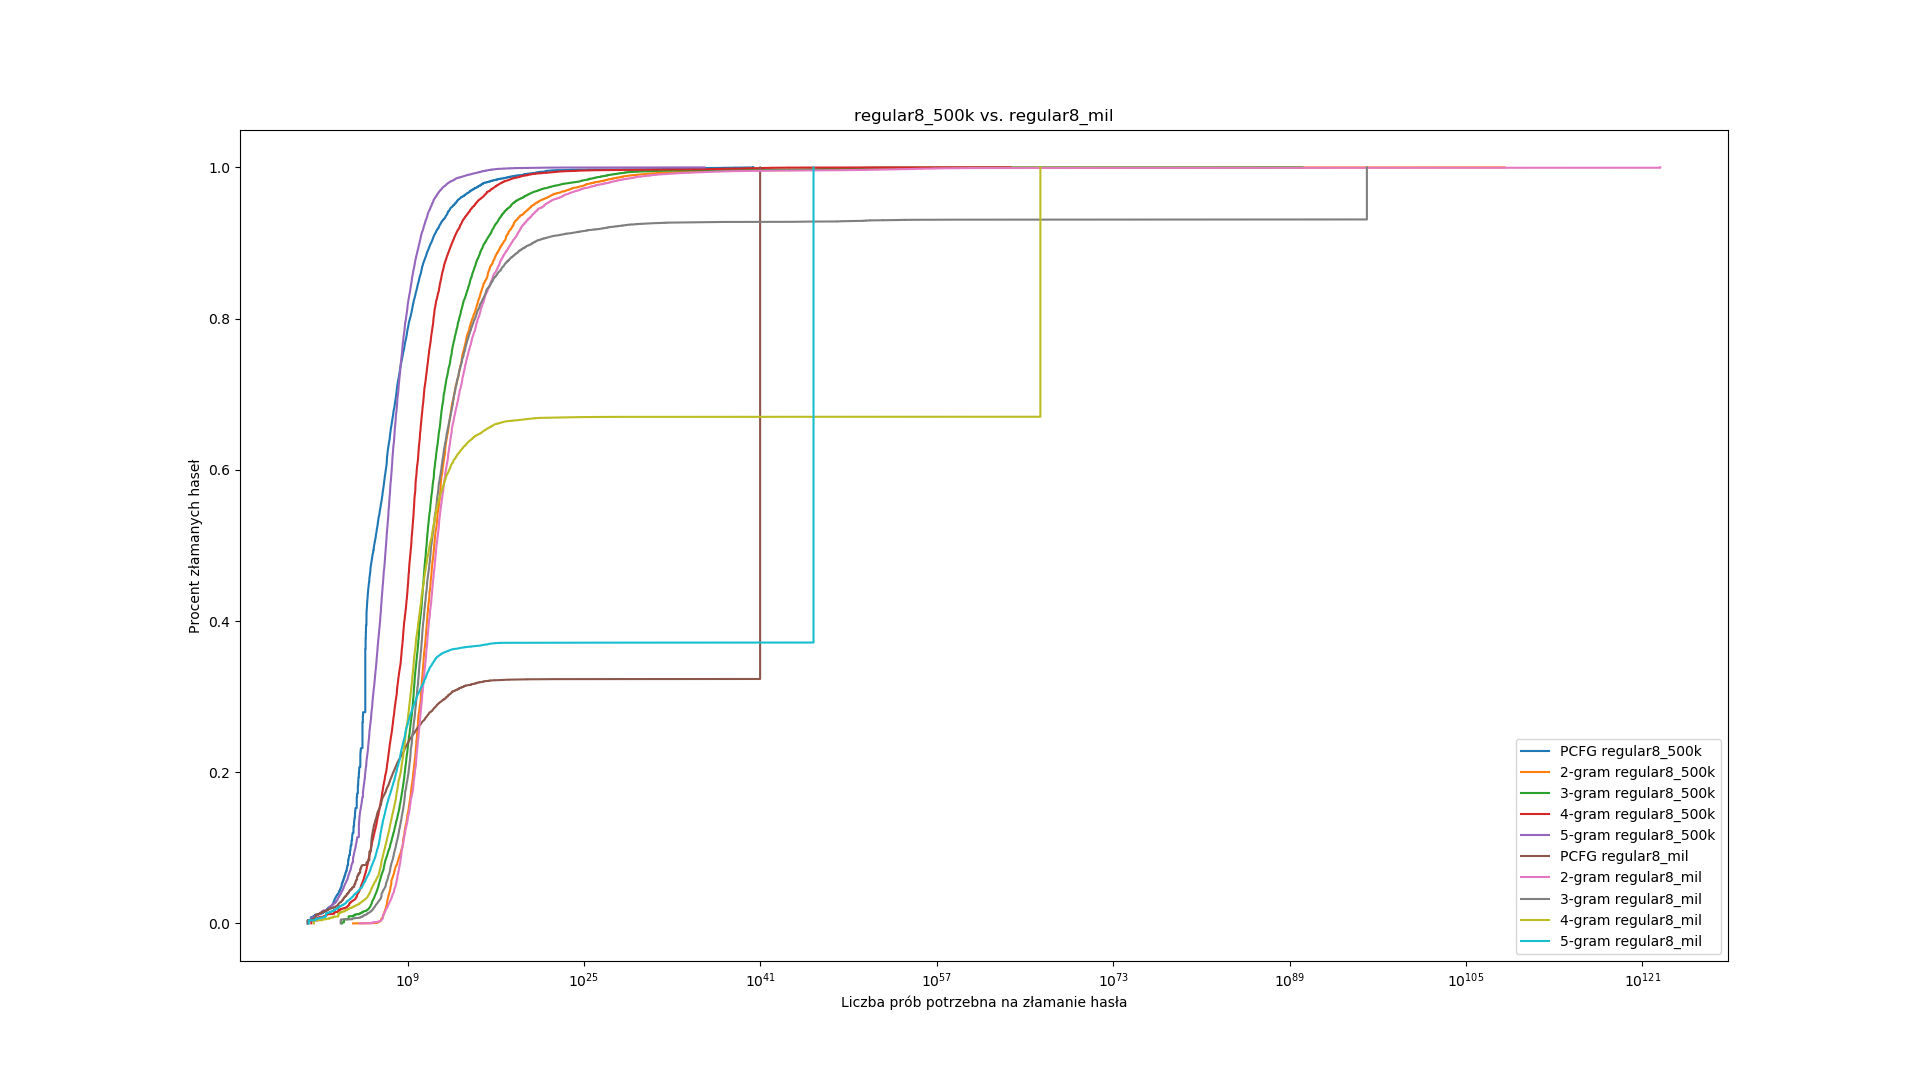
\includegraphics[width=15cm, keepaspectratio]{regular8_500k_regular8_mil}
		\caption{Porównanie polityki regular8 na zbiorze treningowym wielkości 500 tysięcy haseł i wielkości miliona haseł}
	\end{figure}

	\begin{figure}[H]
		\centering
		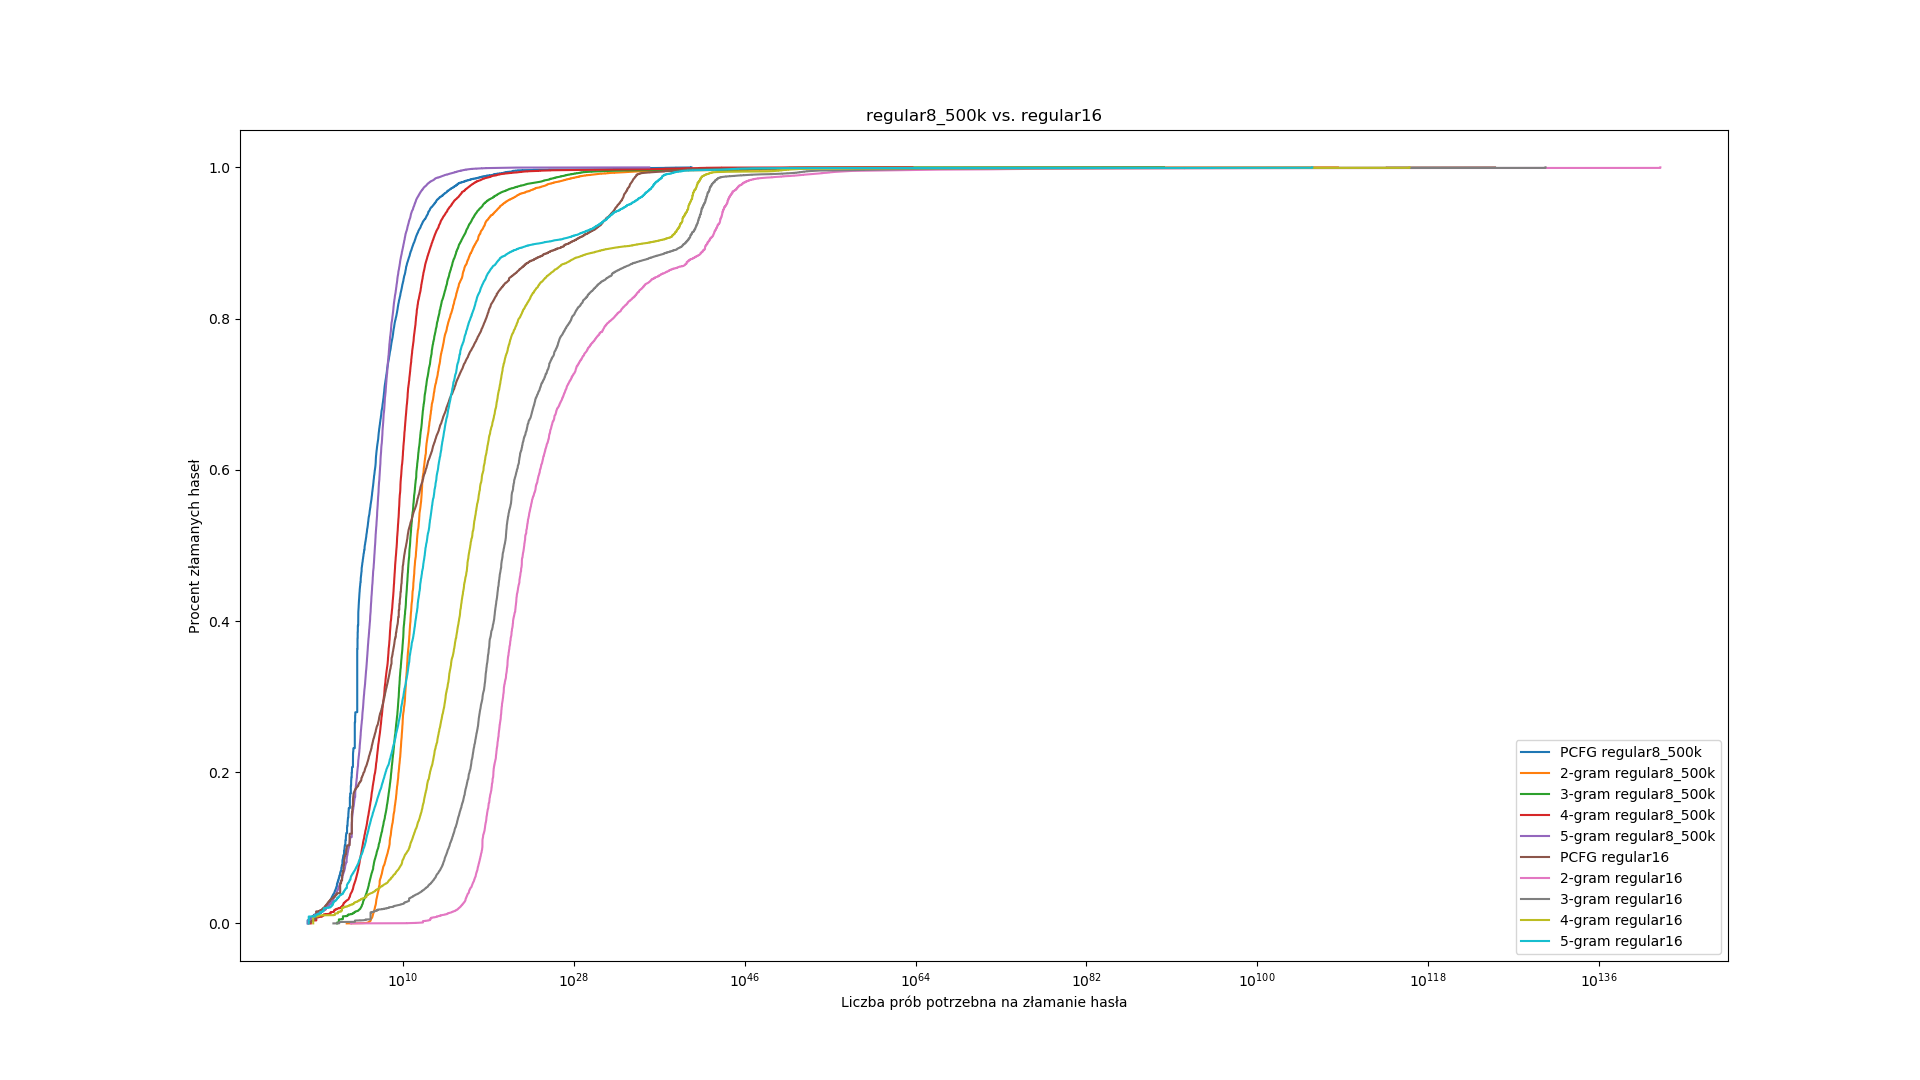
\includegraphics[width=15cm, keepaspectratio]{regular8_500k_regular16}
		\caption{Porównanie polityki regular8 i regular16}
	\end{figure}

	\begin{figure}[H]
		\centering
		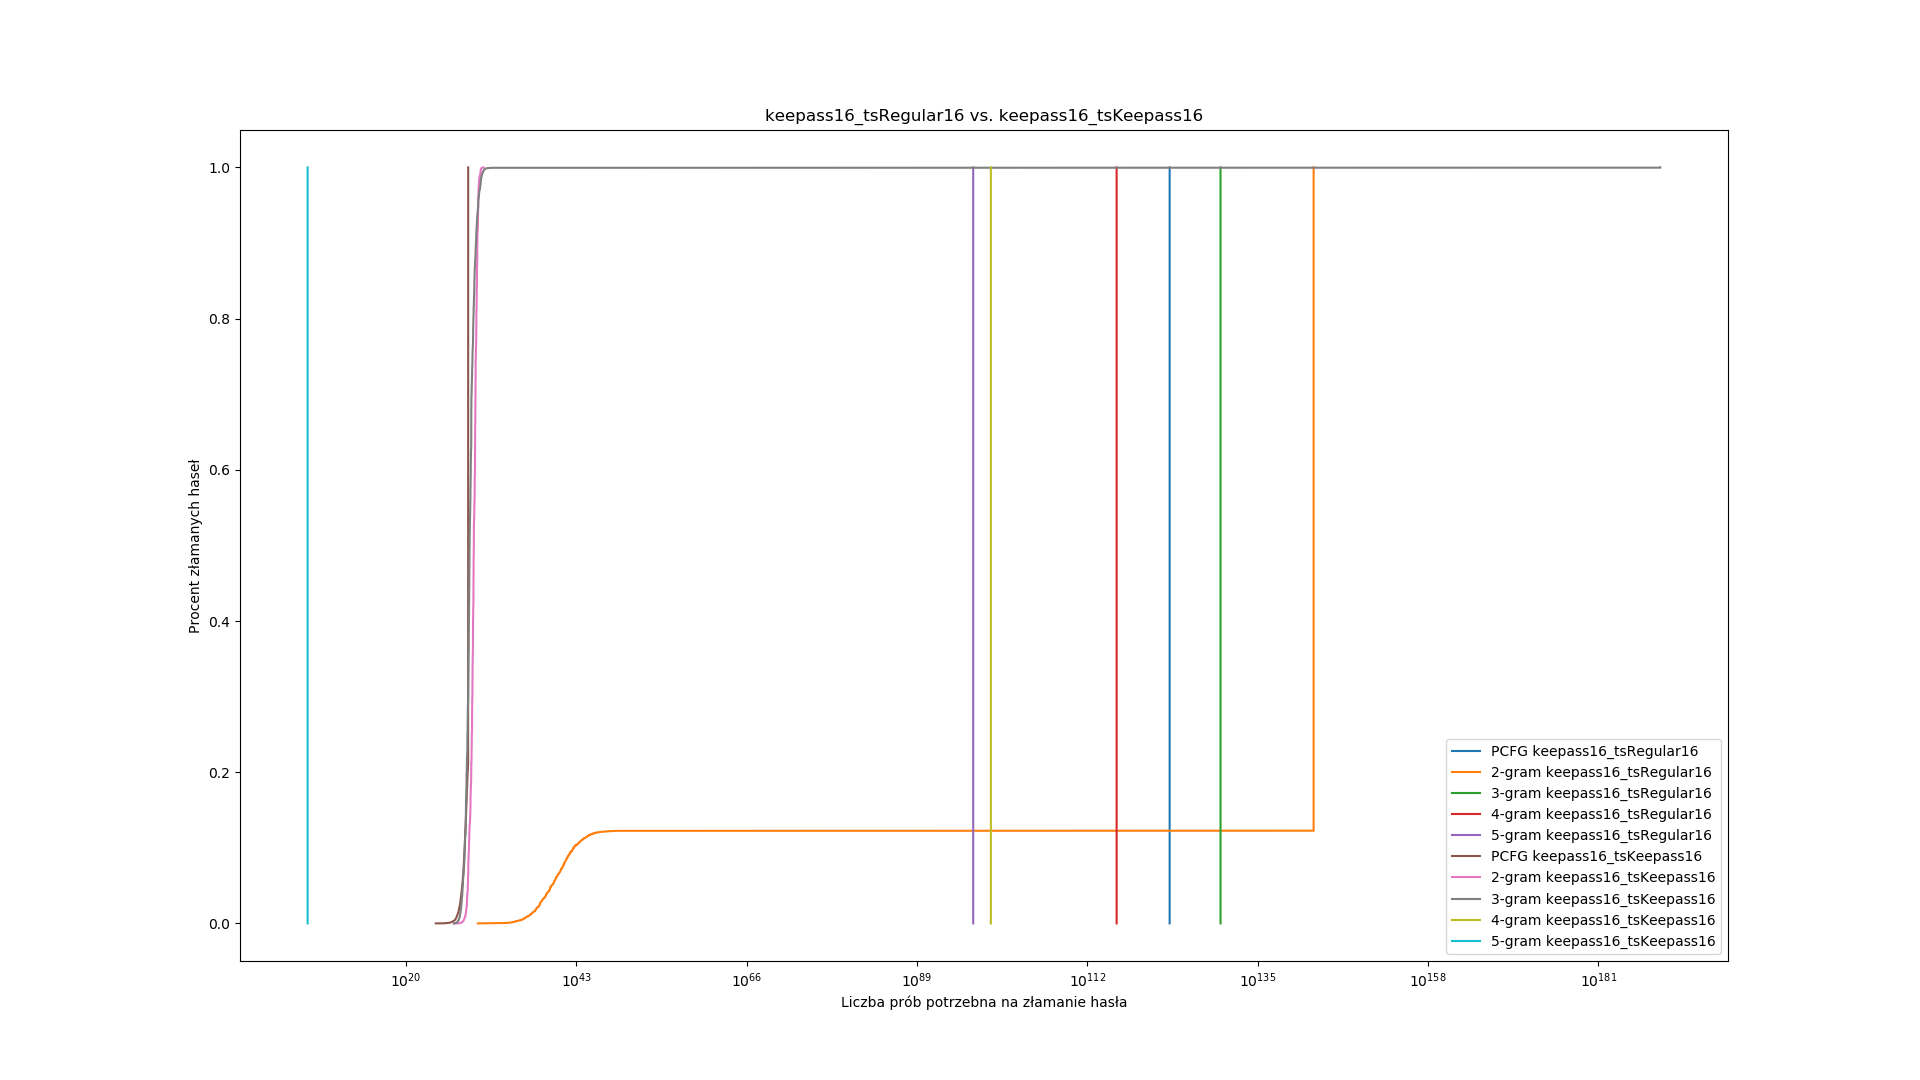
\includegraphics[width=15cm, keepaspectratio]{keepass16_tsRegular16_keepass16_tsKeepass16}
		\caption{Porównanie polityki keepass16 w przypadku zbioru treningowego zawierającego hasła z polityki regular16 i zbioru z hasłami z polity keepass16}
	\end{figure}

	%----------------------------------------------------------------------------------------
	%	SECTION 5
	%----------------------------------------------------------------------------------------
	\newpage
	\section{Analiza wyników}
	\subsection{Analiza wpływu polityki tworzenia haseł i rodzaju używanego algorytmu na skuteczność łamania haseł}
		Przeprowadzone badania potwierdzają zależność pomiędzy stopniem złożoności algorytmu a jego skutecznością
		niezależnie od wybranej polityki tworzenia haseł. Algorytm PCFG, który przeprowadza najbardziej szczegółową
		analizę haseł z ciągu treningowego, wyprzedza w większości polityk wszystkie algorytmy bazujące na n-gramach w liczbie prób, potrzebnych
		do złamania hasła. Podczas porównywania ze sobą n-gramów, również obserwowany jest wpływ długości ciągów znaków
		na skuteczność algorytmu - niezależnie od rodzaju łamanych haseł dłuższy ciąg znaków skutkował większą efektywnością.
		Bardzo zbliżoną skuteczność niezależnie od polityki haseł mają algorytmy PCFG i algorytm bazujący na 5-gramach.
		W przypadku polityk \textit{comprehensive} i \textit{keepass} algorytm oparty na 5-gramach wyprzedza algorytm PCFG.

		Zarówno w przypadku algorytmów opierających się o 2-gramy, jak i 3-gramy, widoczna jest różnica wpływu polityki
		tworzenia haseł na ich siłę (w kontekście ich łamania przez w. w. algorytmy). Hasła, które nie miały żadnych
		zasad regulujących strukturę ich tworzenia, były bardziej podatne na złamanie niż w przypadku polityki \textit{regular8}
		czy \textit{comprehensive8}. Wśród tych dwóch polityk z kolei w około \textit{90\%} przypadków silniejsze były hasła,
		których struktura zawierała minimum jeden znak specjalny, jedną cyfrę i jedną wielką literę. Podobna tendencja widoczna
		jest również w przypadku haseł dwa razy dłuższych - \textit{regular16} i \textit{comprehensive16}.

		W przypadku algorytmów opierających się na 2-gramach i 3-gramach siła haseł w zależności od regorystycznyści polityki
		jest zachowana - najprościej jest złamać hasła bez żadnej polityki, a następnie coraz trudniej kolejno: \textit{regular8},
		\textit{comprehensive8}, \textit{regular16}, \textit{comprehensive16} i najtrudniej \textit{keepass16}. Podobne
		tendencje można zauważyć w przypadku algorytmów opierających się o 4-gramy, jednak hasła z polityki \textit{keepass16}
		jest o wiele trudniej złamać - gdzie w przypadku algorytmu opierającego się o 5-gramy ich siła lekko spada.
		Algorytm PCFG zachowuje podobne prawidłowości w sile haseł w zależności od polityki.

	\subsection{Analiza wpływu wielkości zbioru treningowego na efektywność algorytmów}
		Na rysunku 15 została przedstawiona efektywność algorytmów łamiących hasła z polityki \textit{regular8}, gdzie w jednym
		badaniu algorytmy miały do dyspozycji zbiór treningowy o wielkości 500 tysięcy haseł, a w drugim - miliona haseł. Dzięki nim
		można porównać wpływ wielkości zbioru treningowego na skuteczność algorytmów łamiących hasła. Z badań wynika, że wielkość zbioru
		treningowego faktycznie wpływa na liczbą prób potrzebnych do złamania hasła - dwukrotnie większy zbiór treningowy skutkuje
		dziesięciokrotnym zwiększeniem liczby prób potrzebnych do zgadnięcia hasła.

	\subsection{Analiza wpływu długości haseł na efektywność algorytmów}
		Aby porównać wpływ minimalnej długości hasła na ich siłę, przeprowadzone zostały badania porównujące ze sobą polityki
		\textit{regular8} i \textit{regular16} oraz \textit{comprehensive8} i \textit{comprehensive16}.
		W przypadku polityk \textit{regular8} i \textit{regular16} porównywane są wyniki przedstawione na wykresie 16,
		natomiast w politykach \textit{comprehensive8} i \textit{comprehensive16} na wykresie 14.
		Można dzięki nim zaobserwować, że efektywność algorytmów przy hasłach dwukrotnie dłuższych spada ponad stukrotnie -
		drastycznie wzrasta liczba prób potrzebnych do złamania hasła niezależnie od wykorzystanego algorytmu.

	\subsection{Analiza wpływu rodzaju haseł zawartych w ciągu treningowym na efektywność algorytmów}
		Na podstawie rysunku 17 porównywana jest siła haseł w polityce \textit{keepass16} w przypadku uczenia algorytmów
	na dwóch różnych zbiorach treningowych - jednym opartym o hasła z tej polityki i drugim opartym o hasła z polityki \textit{regular16}.
	Zazwyczaj osoby, które mają na celu złamanie jakiegoś hasła, uwzględniają w zbiorze treningowym politykę tworzenia haseł w serwisie.
	W regułach tworzenia haseł w serwisie wymagania mogą być sprecyzowane co do długości hasła czy liczby znaków specjalnych,
	natomiast osoba łamiąca hasło najpewniej nie ma świadomości czy dane hasło jest słownikowe czy losowo generowane,
	więc najprawdopodobniej jako zbiór treningowy użyje zbioru haseł zawierających wszystkie rodzaje haseł spełniające wymagania serwisu.

	Dzięki przeprowadzonym badaniom można zauważyć, że niezależnie od wybranego algorytmu zbiór uczący zawierający hasła z polityki,
	która odpowiada polityce łąmanego hasła, czyli \textit{keepass16 tsKeepass16}, oferuje lepszą skuteczność łamania haseł
	niż zbiór treningowy składający się z haseł z innej polityki. Z punktu widzenia osoby łąmiącej hasła najlepsze wyniki może osiągnąć
	znając jak najwięcej informacji o strukturze łamanego hasła - jego długości, zawartych w nim znaków czy jego znaczenia. Dzięki takim informacjom
	może lepiej dobrać zbiór treningowy i osiągnąć większą skuteczność w łamaniu haseł. Z punktu widzenia osoby tworzącej hasło
	lepiej jest używać haseł generowanych losowo, ponieważ - o ile osoba potencjalnie łąmiąca hasło, nie ma świadomości, że hasło jest
	generowane losowo - takie hasła są wielokrotnie silniejsze w kontekście ich łamania.


	%----------------------------------------------------------------------------------------
	%	SECTION 6
	%----------------------------------------------------------------------------------------
	%\newpage
	\section{Podsumowanie}
	Przeprowadzone badania potwierdziły słuszność najpopularniejszych polityk tworzenia haseł uznawanych za skuteczne. Hasła dłuższe i
	zawierające znaki specjalne są trudniejsze do złamania, choć najbezpieczniejszą metodą tworzenia haseł są jest ich losowe generowanie.
	Niezależnie od wykorzystanego algorytmu łamiącego hasła są one nieporównywalnie silniejsze, a większość osób łamiących hasła dysponuje
	ciągiem treningowym w postaci zbioru zawierającego hasła tworzone ze słów. W analizowanej bazie haseł można jednak znaleźć ogromną
	liczbę haseł, które są bardzo proste i przewidywalne, co wskazuje na niedbałość lub nieświadomość osób zabezpieczających swoje konta.

	Efektywność badanych algorytmów do łamania haseł rośnie wraz ze stopniem ich złożoności. Czym więcej operacji analizujących ciąg treningowy
	musi zostać wykonanych podczas pracy algorytmu, tym mniej prób potrzeba, aby hasło zostało złamane. Na skuteczność algorytmu ma duży wpływ
	wielkość ciągu treningowego oraz odpowiednia kategoria haseł w nim zawarta - szybciej złamane zostaną hasła, które odpowiadają polityką
	tym zawartym w ciągu treningowym. Osoba łamiąca hasła może zyskać największą przewagę znając jak najwięcej informacji o strukturze
	łamanego hasła (jego długości, zawieranych znaków, losowości lub znaczenia), ponieważ dzięki temu może dobrze dopasować ciąg treningowy,
	a tym samym uzyskać najlepsze rezultaty.

	%----------------------------------------------------------------------------------------
	\newpage
	\bibliography{bibliography}
	
\end{document}